\documentclass{beamer}
\usepackage{tikz}
\usepackage{gillius}
\usepackage{abraces}
\usepackage{etex}
\usepackage{array}
\usepackage{multirow}
\usepackage{qrcode}
\usepackage[backend=biber, style=authoryear, uniquelist=minyear, uniquename=false]{biblatex}

% http://tex.stackexchange.com/questions/12703/how-to-create-fixed-width-table-columns-with-text-raggedright-centered-raggedlef
\newcolumntype{L}[1]{>{\raggedright\let\newline\\\arraybackslash\hspace{0pt}}m{#1}}
\newcolumntype{C}[1]{>{\centering\let\newline\\\arraybackslash\hspace{0pt}}m{#1}}
\newcolumntype{R}[1]{>{\raggedleft\let\newline\\\arraybackslash\hspace{0pt}}m{#1}}

\usetikzlibrary{external}
\usetikzlibrary{shapes}
\usetikzlibrary{arrows}
\usetikzlibrary{positioning}
\usetikzlibrary{decorations.pathreplacing}

\usetheme[everytitleformat=regular]{m}
\setbeamertemplate{navigation symbols}{}

\graphicspath{{../figures/}}
\newcommand{\tablepath}{../tables}

\title{Phylogenetic inference of contact network parameters with kernel approximate Bayesian computation}
\author[RMM, RHL \& AFYP]{Rosemary M McCloskey$^1$ \and Richard H Liang$^1$ \and Art FY Poon$^{1,2}$}
\institute[UBC \& BCCfE]{$^1$BC Centre for Excellence in HIV/AIDS, Vancouver, Canada \\ $^2$Department of Medicine, University of British Columbia, Vancouver, Canada}
\date{HIV Dynamics \& Evolution, Woods Hole, USA, April 25, 2016}

\newcommand{\dd}[2]{\frac{\text{d}\,#1}{\text{d}\,#2}}

\addbibresource{papers.bib}

\begin{document}
\setbeamercolor{background canvas}{bg=white}
\renewcommand{\footnotesize}{\tiny}
\definecolor{red}{RGB}{228,26,28}
\definecolor{blue}{RGB}{55,126,184}
\definecolor{green}{RGB}{77,175,74}
\definecolor{purple}{RGB}{152,78,163}

\maketitle

\begin{frame}{Most epidemiological models assume homogeneous mixing}
  \begin{columns}
    \begin{column}{0.6\textwidth}
      \centering
      \includegraphics[scale=0.6]{compartments}
      \vspace{1cm}

      \uncover<3->{\includegraphics[width=\textwidth]{sir-trajectories}}
    \end{column}
    \begin{column}{0.4\textwidth}
      \vspace{-2cm}
      \begin{itemize}
        \setlength{\itemsep}{24pt}
        \uncover<2->{
        \item Often provide a reasonable approximation in practice.
        }
        \uncover<3->{
        \item Can be inaccurate when substantial contact heterogeneity exists.
        }
      \end{itemize}
    \end{column}
  \end{columns}
\end{frame}

\begin{frame}{Network models capture contact heterogeneity}
  \begin{columns}
    \begin{column}{0.5\textwidth}
      \includegraphics[width=\textwidth]{contactnet-empty}
    \end{column}
    \begin{column}{0.5\textwidth}
      \begin{itemize}
        \setlength{\itemsep}{12pt}
          \pause
        \item May offer more accurate predictions for highly structured
          populations.
          \pause
        \item Network parameters may be of interest for their own sake,
          \textit{e.g.} are there superspreaders?
          \pause
        \item Extremely difficult to estimate in practice.
      \end{itemize}
    \end{column}
  \end{columns}

\end{frame}

\begin{frame}{Contact networks shape transmission trees}
  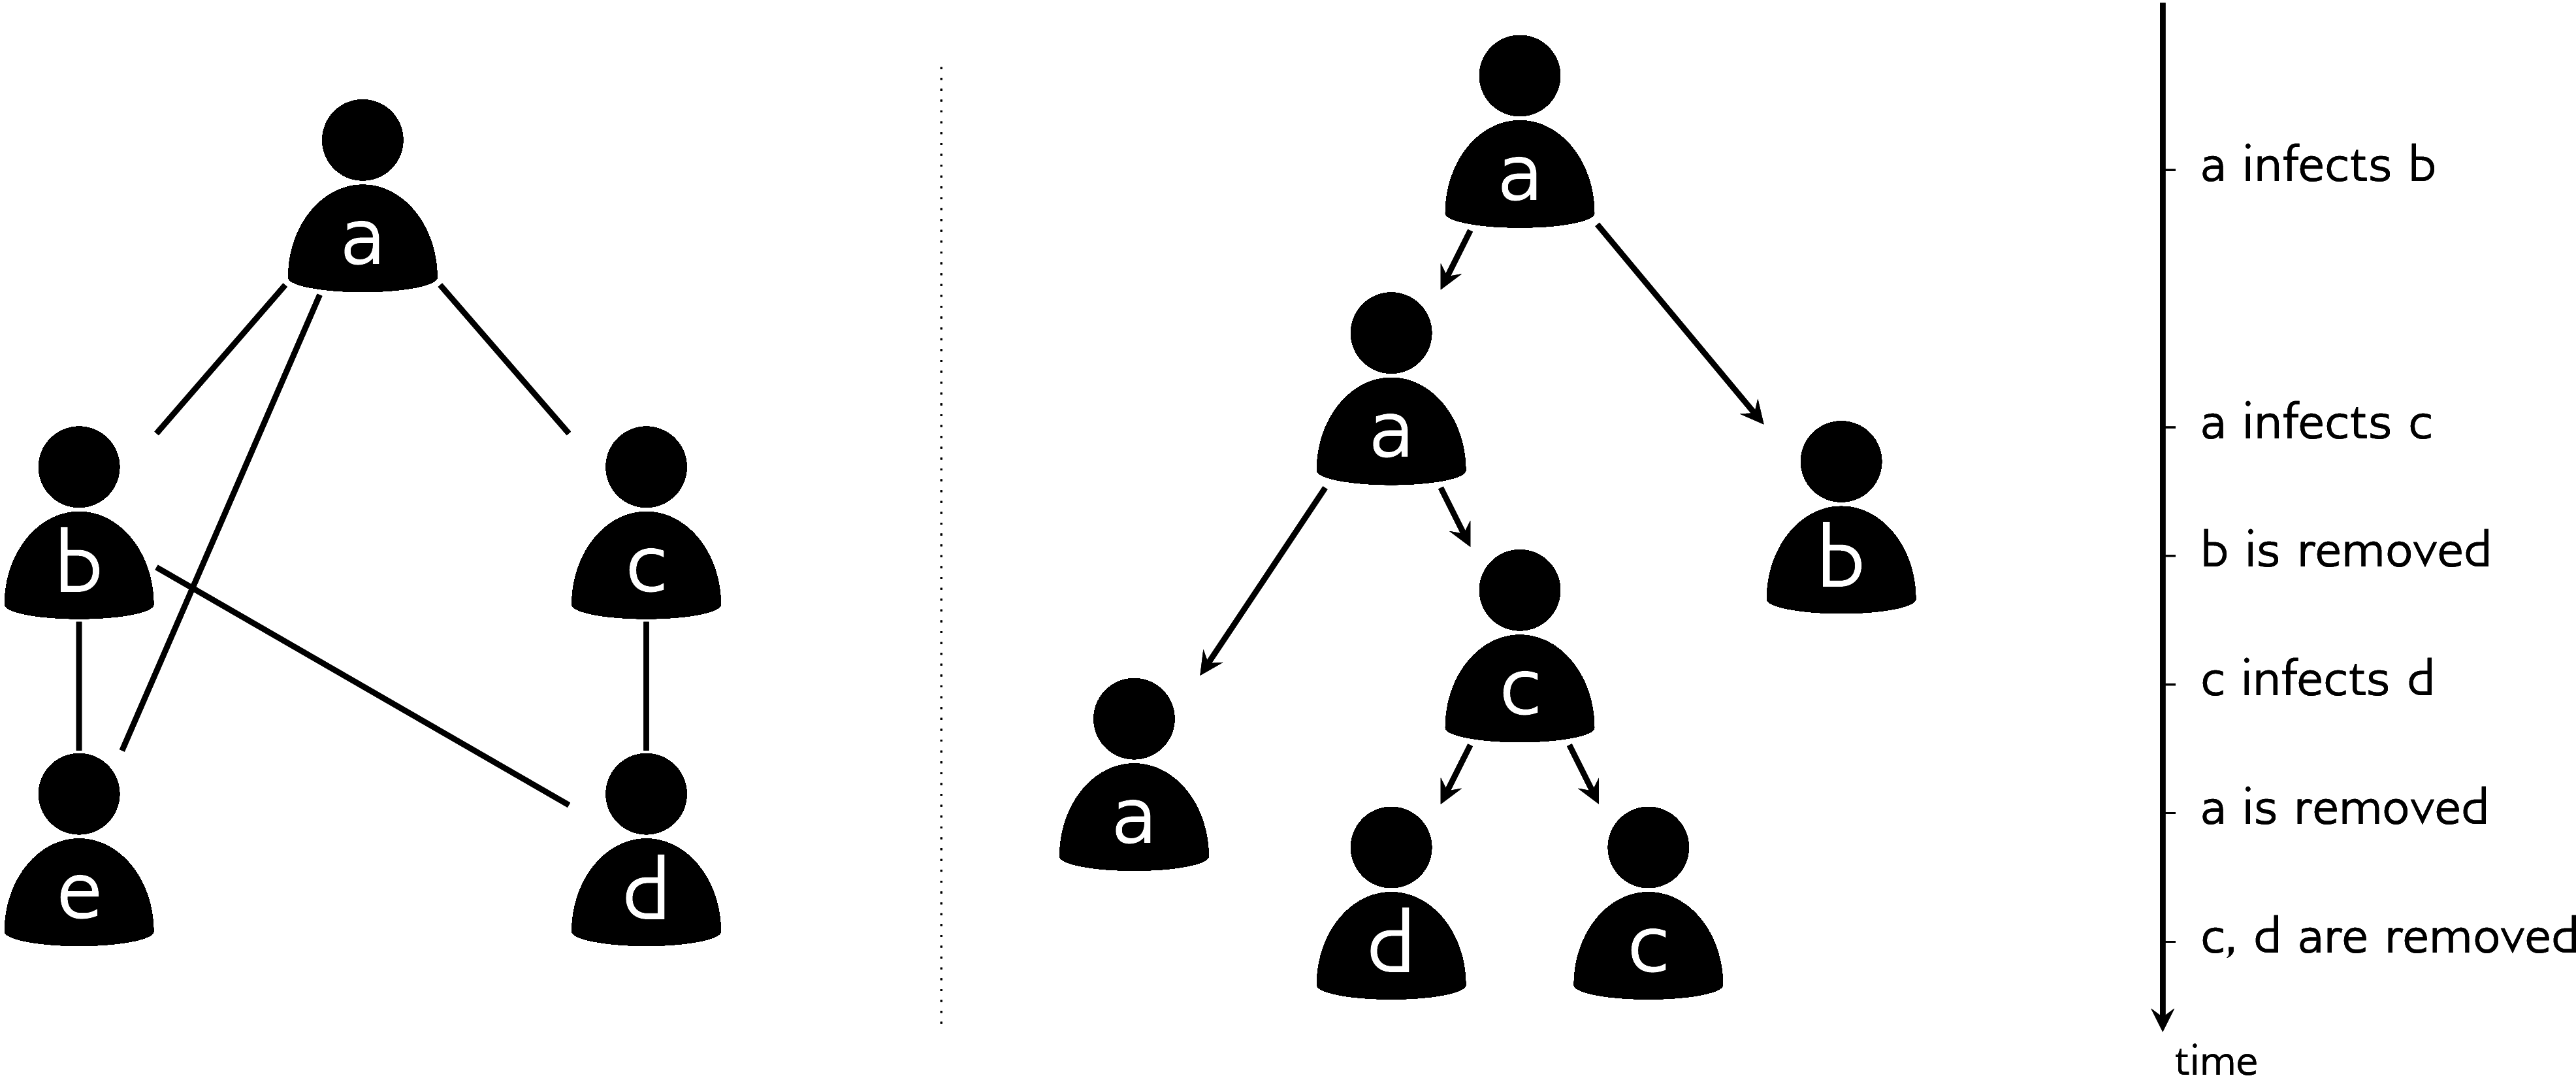
\includegraphics[width=\textwidth]{contactnet}

  \begin{itemize}
      \pause
    \item Transmission trees in turn shape viral phylogenies.
      \pause
    \item \textbf{Aim:} estimate contact network parameters from viral
      phylogenies.
  \end{itemize}
\end{frame}

%\begin{frame}{Preferential attachment generates scale-free networks}
%  \includegraphics[width=\textwidth]{pa-example}
%  \begin{itemize}
%    \item Sexual networks are often scale-free: degree distributions appear
%      follow a power law ($\Pr(\text{degree} = d) \propto d^{-\gamma}$).
%      \pause
%    \item Preferential attachment models generate scale-free networks.
%  \end{itemize}
%\end{frame}

\begin{frame}{Barab\'asi-Albert model incorporates preferential attachment}
  \begin{columns}
    \begin{column}{0.5\textwidth}
      \begin{minipage}[p][\textheight][t]{\textwidth}
        \centering
        \only<1>{\includegraphics[page=1, width=\textwidth]{pa.pdf}}
        \only<2>{\includegraphics[page=2, width=\textwidth]{pa.pdf}}
        \only<3>{\includegraphics[page=3, width=\textwidth]{pa.pdf}}
        \only<4>{\includegraphics[page=4, width=\textwidth]{pa.pdf}}
        \only<5>{\includegraphics[page=5, width=\textwidth]{pa.pdf}}
        \only<6>{\includegraphics[page=6, width=\textwidth]{pa.pdf}}
      \end{minipage}
    \end{column}
    \begin{column}{0.5\textwidth}
      \begin{minipage}[t][\textheight][t]{\textwidth}
      \begin{itemize}
        \uncover<1->{ \item Start with a small number of connected nodes. }
        \uncover<2->{ \item Attach new nodes with $m$ edges. }
        \uncover<3->{ \item Other endpoints of degree $d$ are chosen with probability $\propto d^{\alpha} + 1$. }
        \uncover<5->{ \item Continue until network has $N$ nodes. }
        \uncover<6->{ \item Also consider the prevalence $I$. }
      \end{itemize}
      \end{minipage}
    \end{column}
  \end{columns}
\end{frame}

\begin{frame}{Do network parameters measurably affect tree shape?}
  \only<1>{
    \includegraphics[height=1in, trim=0 2in 4in 0, clip]{kernel-idea}
  }
  \only<2>{
    \includegraphics[height=1in, trim=0 2in 2in 0, clip]{kernel-idea}
  }
  \only<3->{
    \includegraphics[height=1in, trim=0 2in 0 0, clip]{kernel-idea}
  }
  \begin{itemize}
    \setlength{\itemsep}{0pt}
    \item Generate networks under different parameter values (number of nodes
      $N$, number of edges per vertex $m$, pereferential attachment power
      $\alpha$).
    \uncover<2->{
    \item Simulate epidemic over each network until $I$ nodes are infected.
    }
    \uncover<3->{
    \item Randomly subsample to form transmission trees.
    }
    \uncover<4->{
    \item Compare trees pairwise using tree kernel\footfullcite{poon2013mapping}.
    }
  \end{itemize}
\end{frame}

\begin{frame}{Preferential attachment power $\alpha$ affects tree shape}
  \begin{tikzpicture}[remember picture, overlay]
    \node at (current page.south west) [anchor=south west] {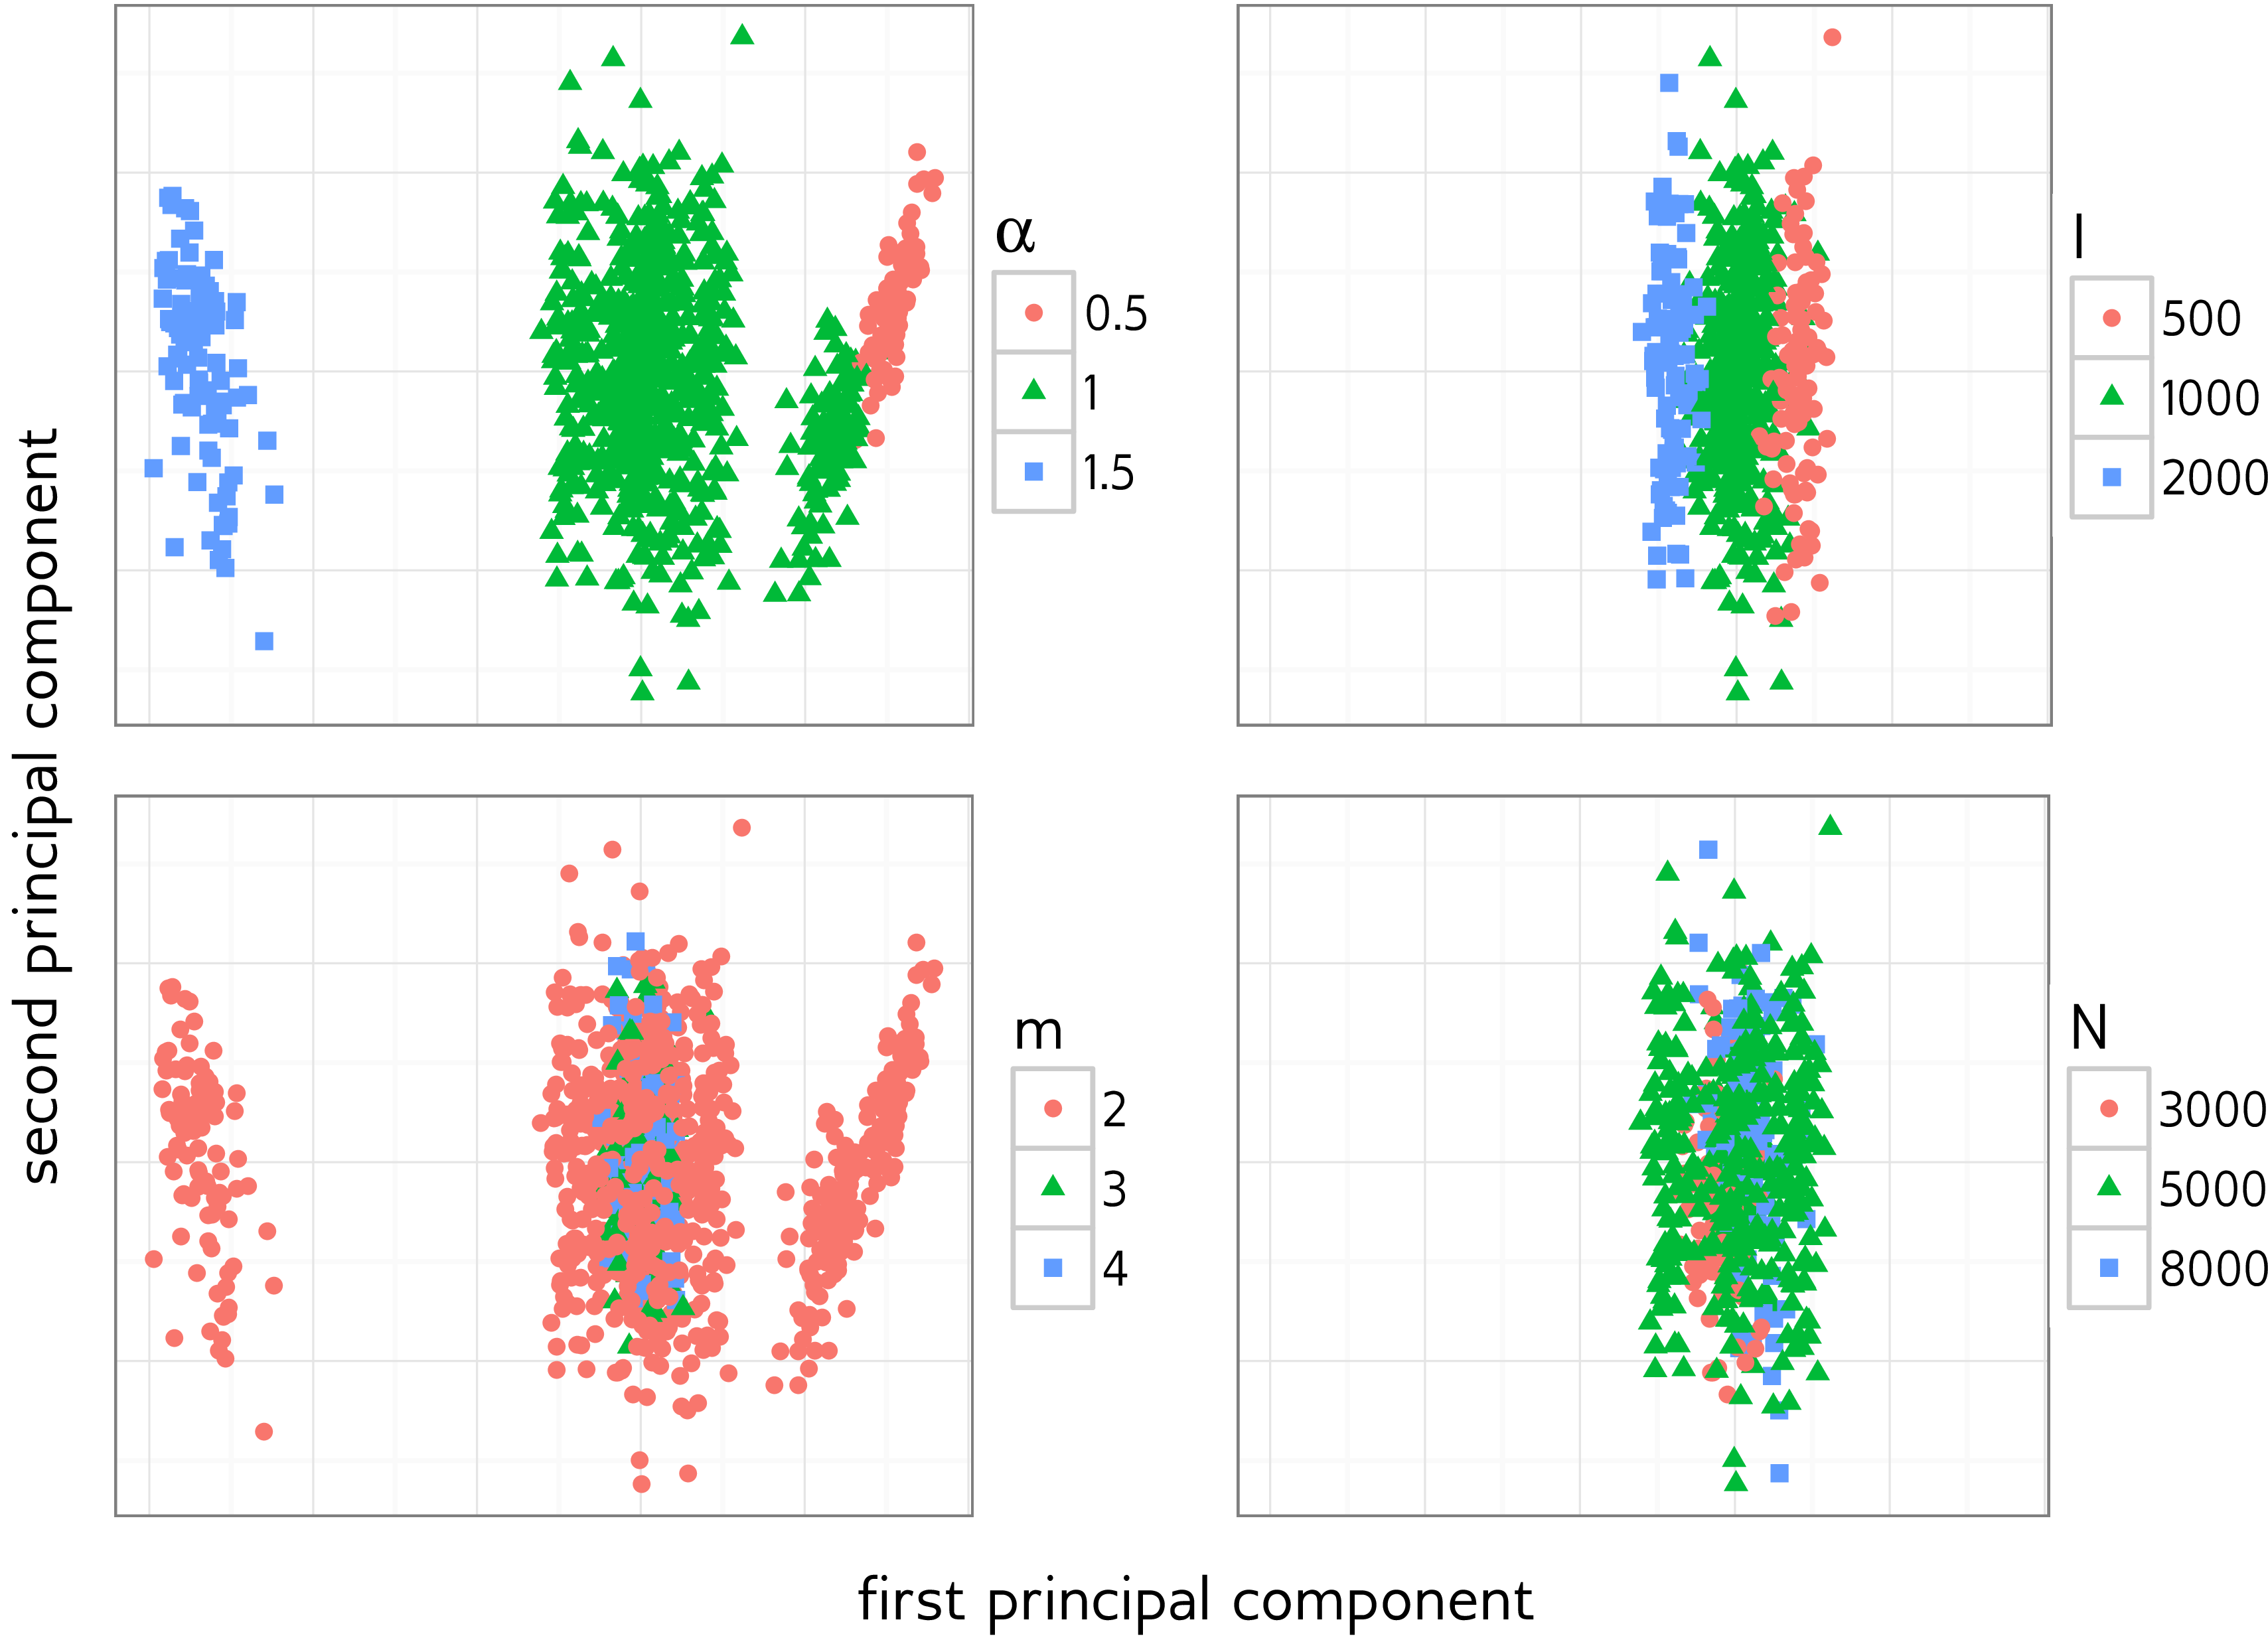
\includegraphics[width=0.6\textwidth, trim=0.2in 2.7in 3.3in 0, clip]{kernel-kpca.pdf}};
    \node (t) at (current page.north east) [anchor=north east, inner ysep=1.5cm, inner xsep=0.5cm] {\includegraphics[width=0.7\textwidth]{kernel-alpha-tree.pdf}};
  \end{tikzpicture}
\end{frame}

\begin{frame}{Prevalence $I$ affects tree shape}
  \begin{tikzpicture}[remember picture, overlay]
    \node at (current page.south west) [anchor=south west] {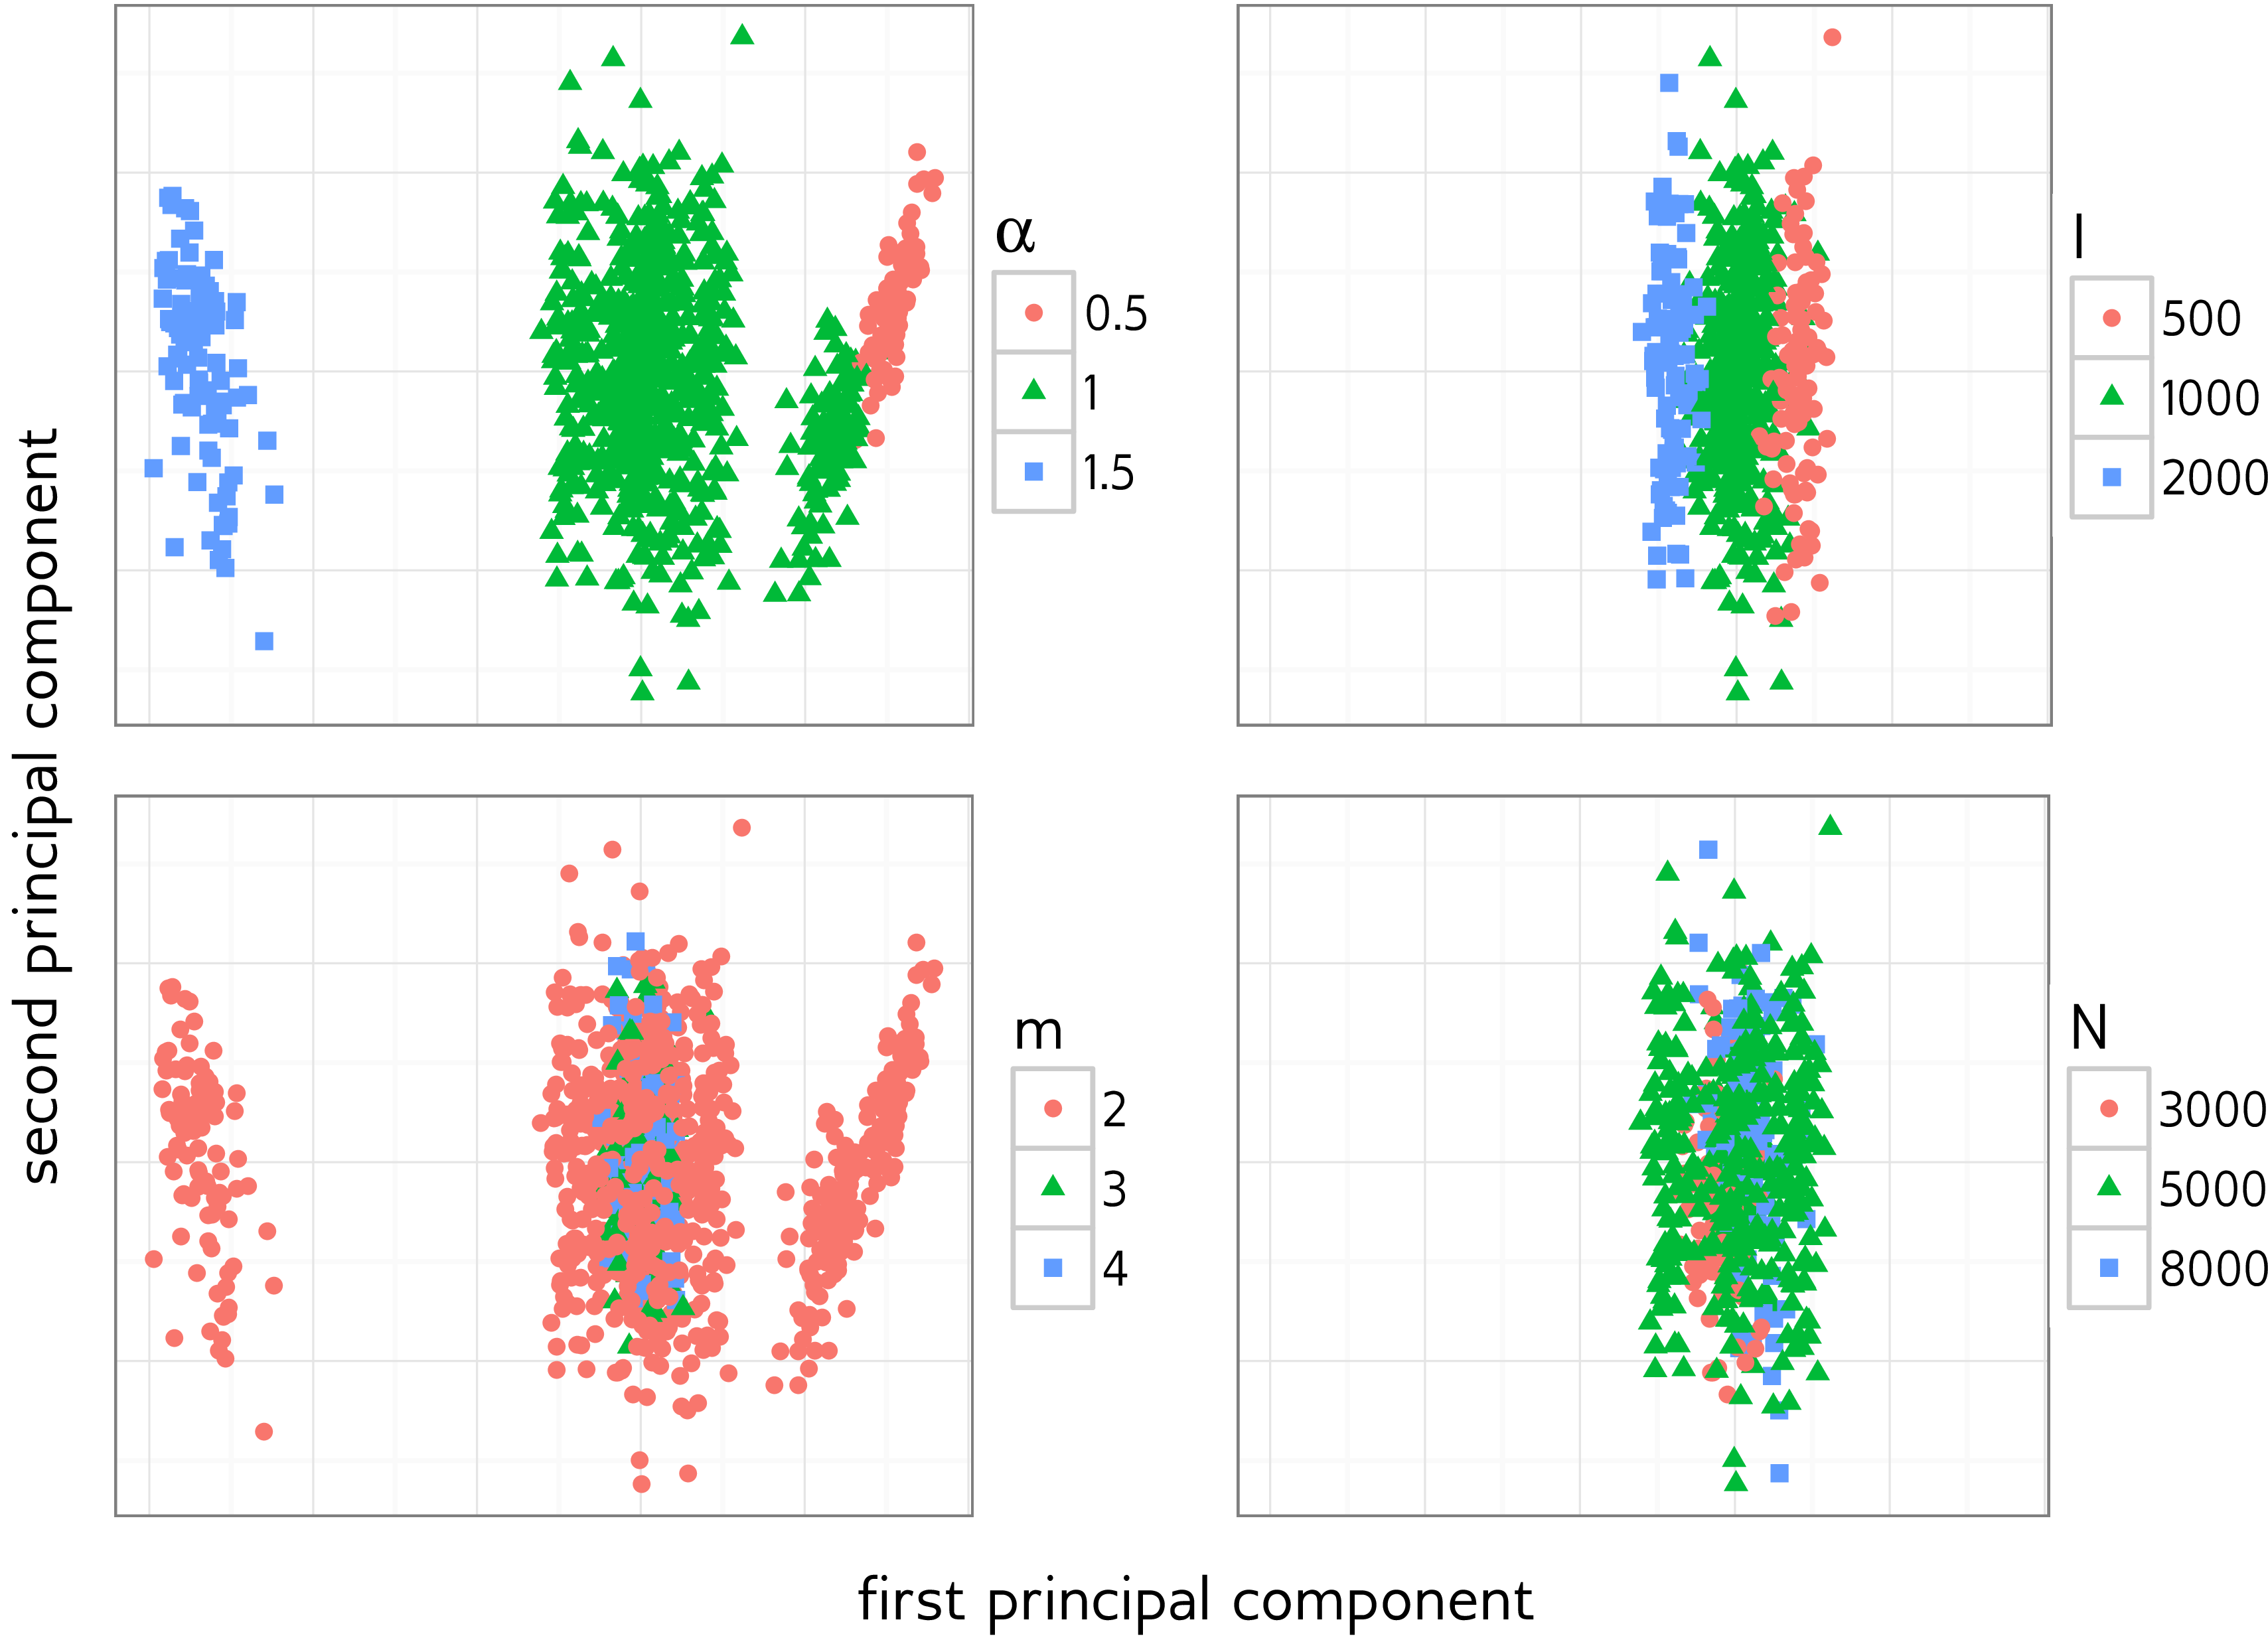
\includegraphics[width=0.6\textwidth, trim=3.5in 2.7in 0in 0, clip]{kernel-kpca.pdf}};
    \node (t) at (current page.north east) [anchor=north east, inner ysep=1.5cm, inner xsep=0.5cm] {\includegraphics[width=0.7\textwidth]{kernel-I-tree.pdf}};
  \end{tikzpicture}
\end{frame}

\begin{frame}{Number of edges per vertex $m$ does not affect tree shape}
  \begin{tikzpicture}[remember picture, overlay]
    \node at (current page.south west) [anchor=south west] {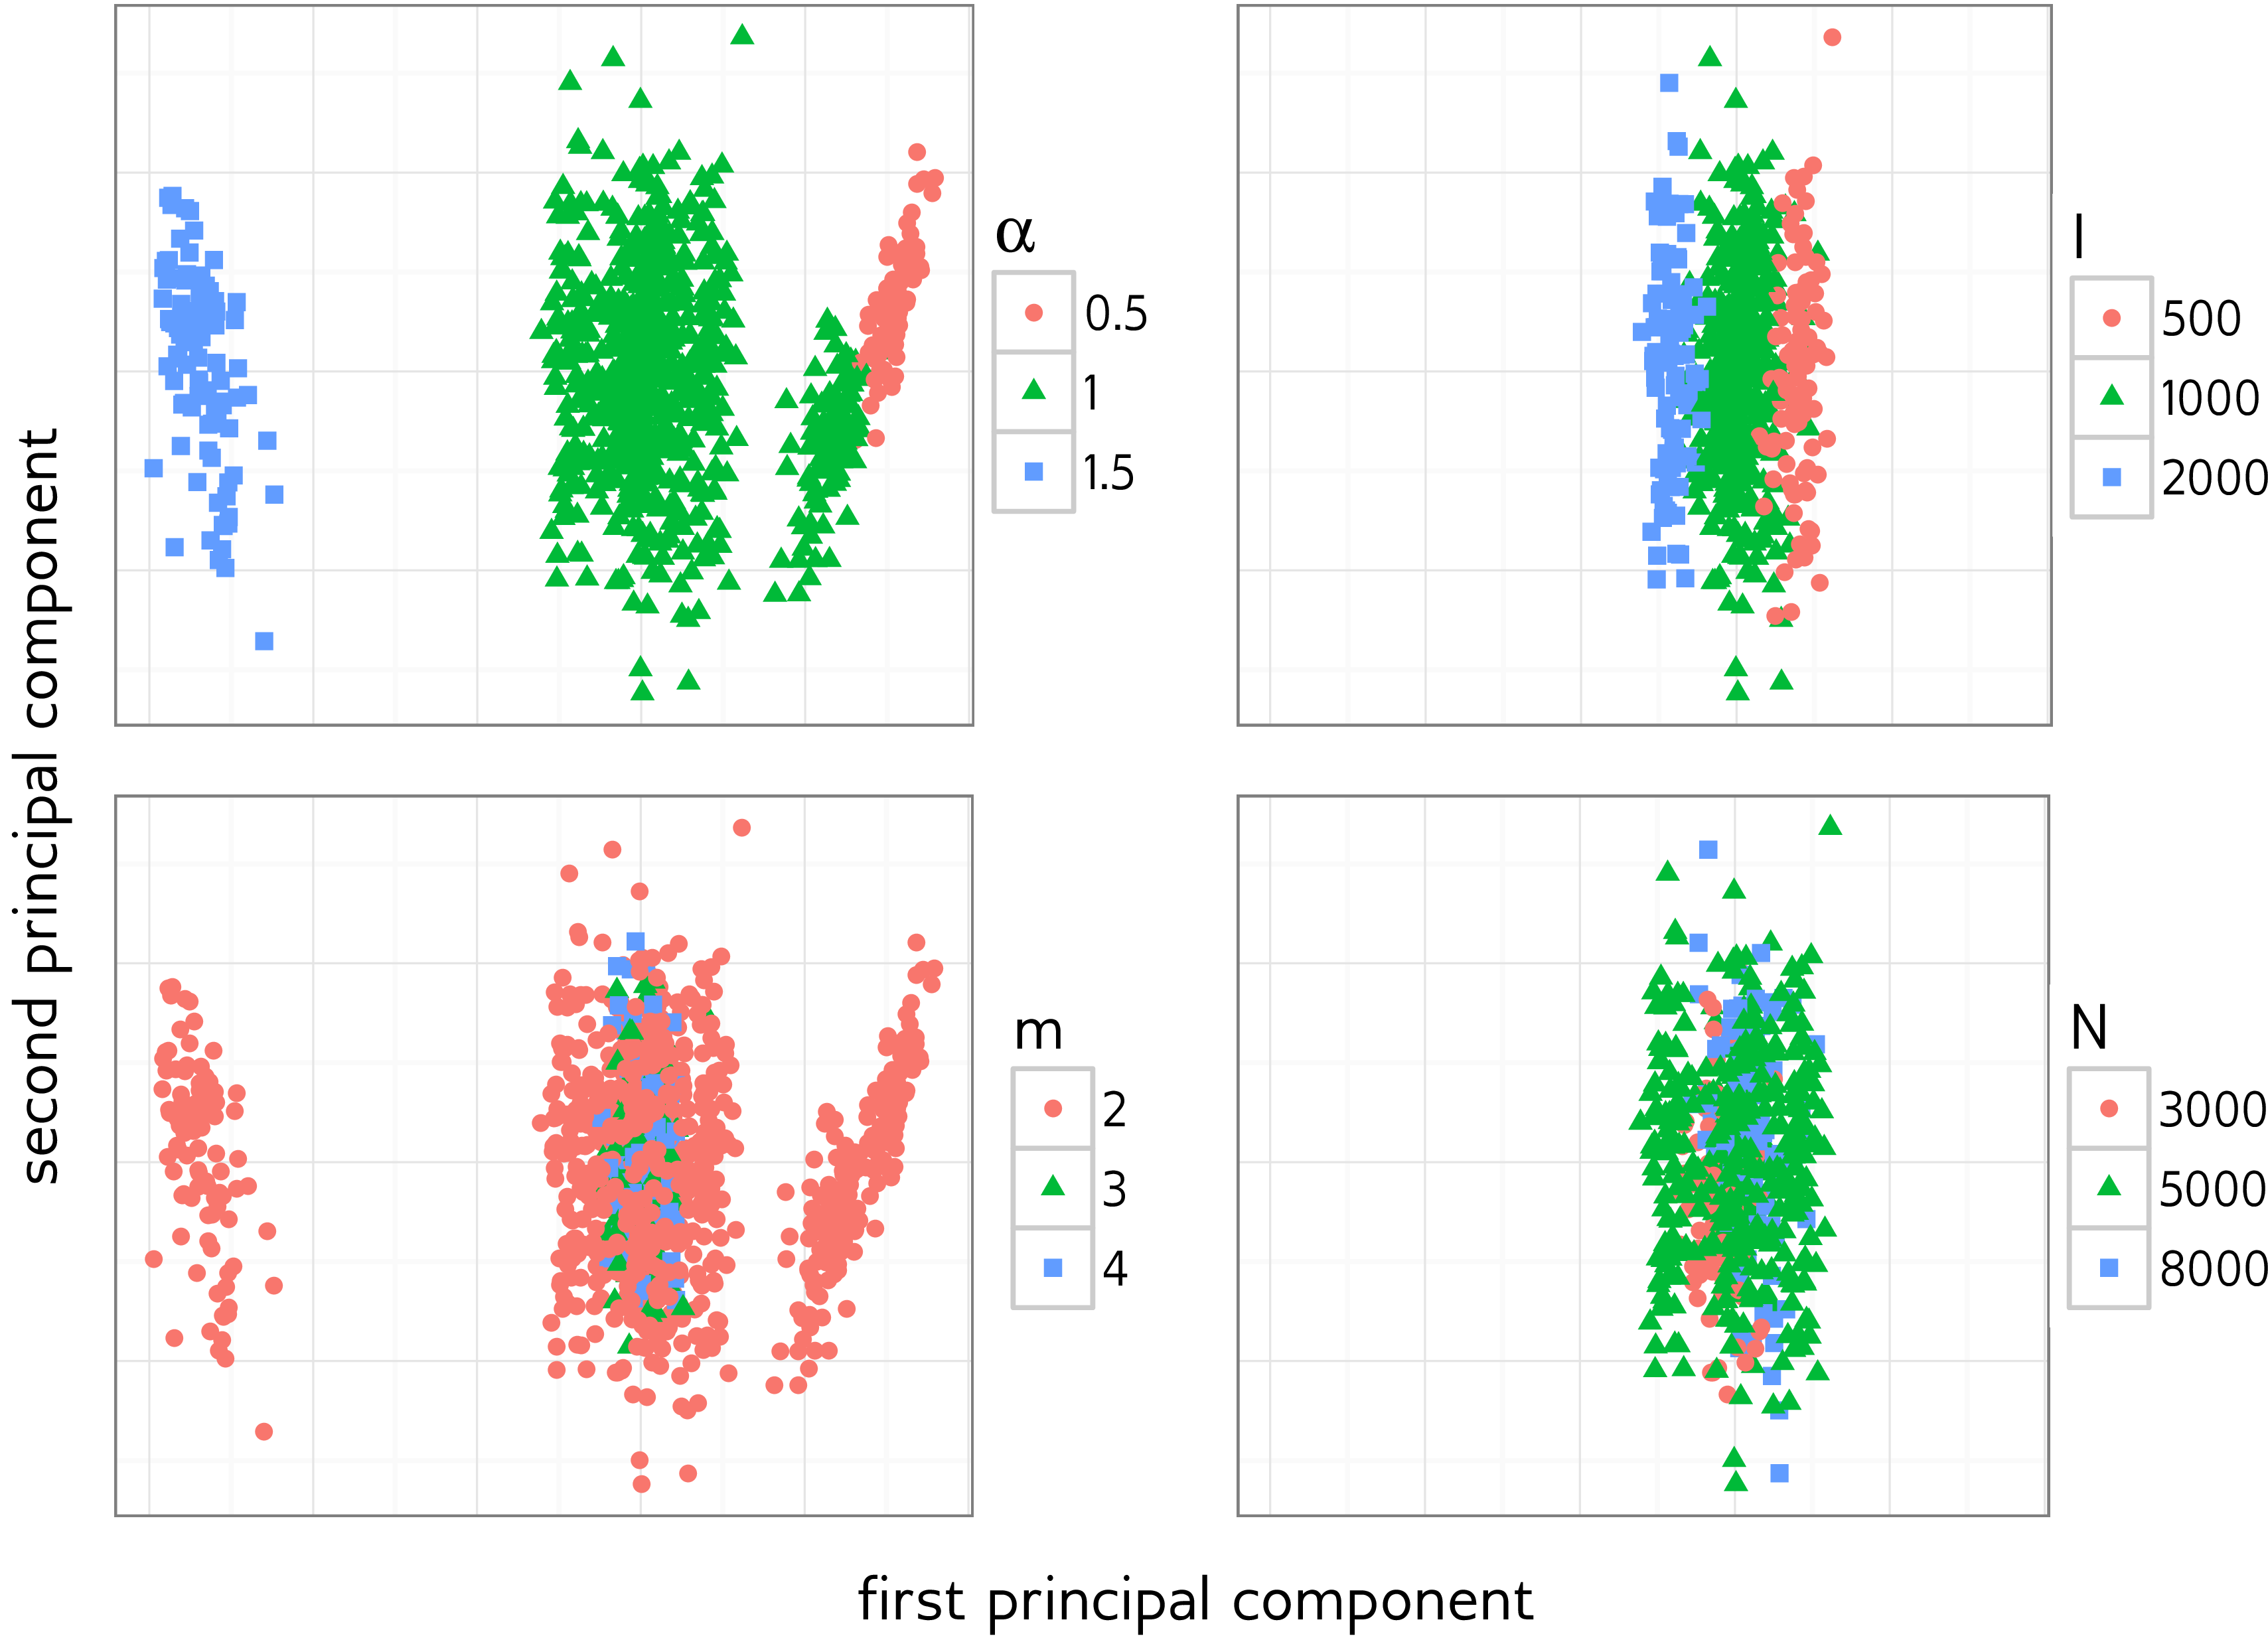
\includegraphics[width=0.6\textwidth, trim=0.2in 0.3in 3.3in 2.2in, clip]{kernel-kpca.pdf}};
    \node (t) at (current page.north east) [anchor=north east, inner ysep=1.5cm, inner xsep=0.5cm] {\includegraphics[width=0.7\textwidth]{kernel-m-tree.pdf}};
  \end{tikzpicture}
\end{frame}

\begin{frame}{Number nodes $N$ modestly affects tree shape}
  \begin{tikzpicture}[remember picture, overlay]
    \node at (current page.south west) [anchor=south west] {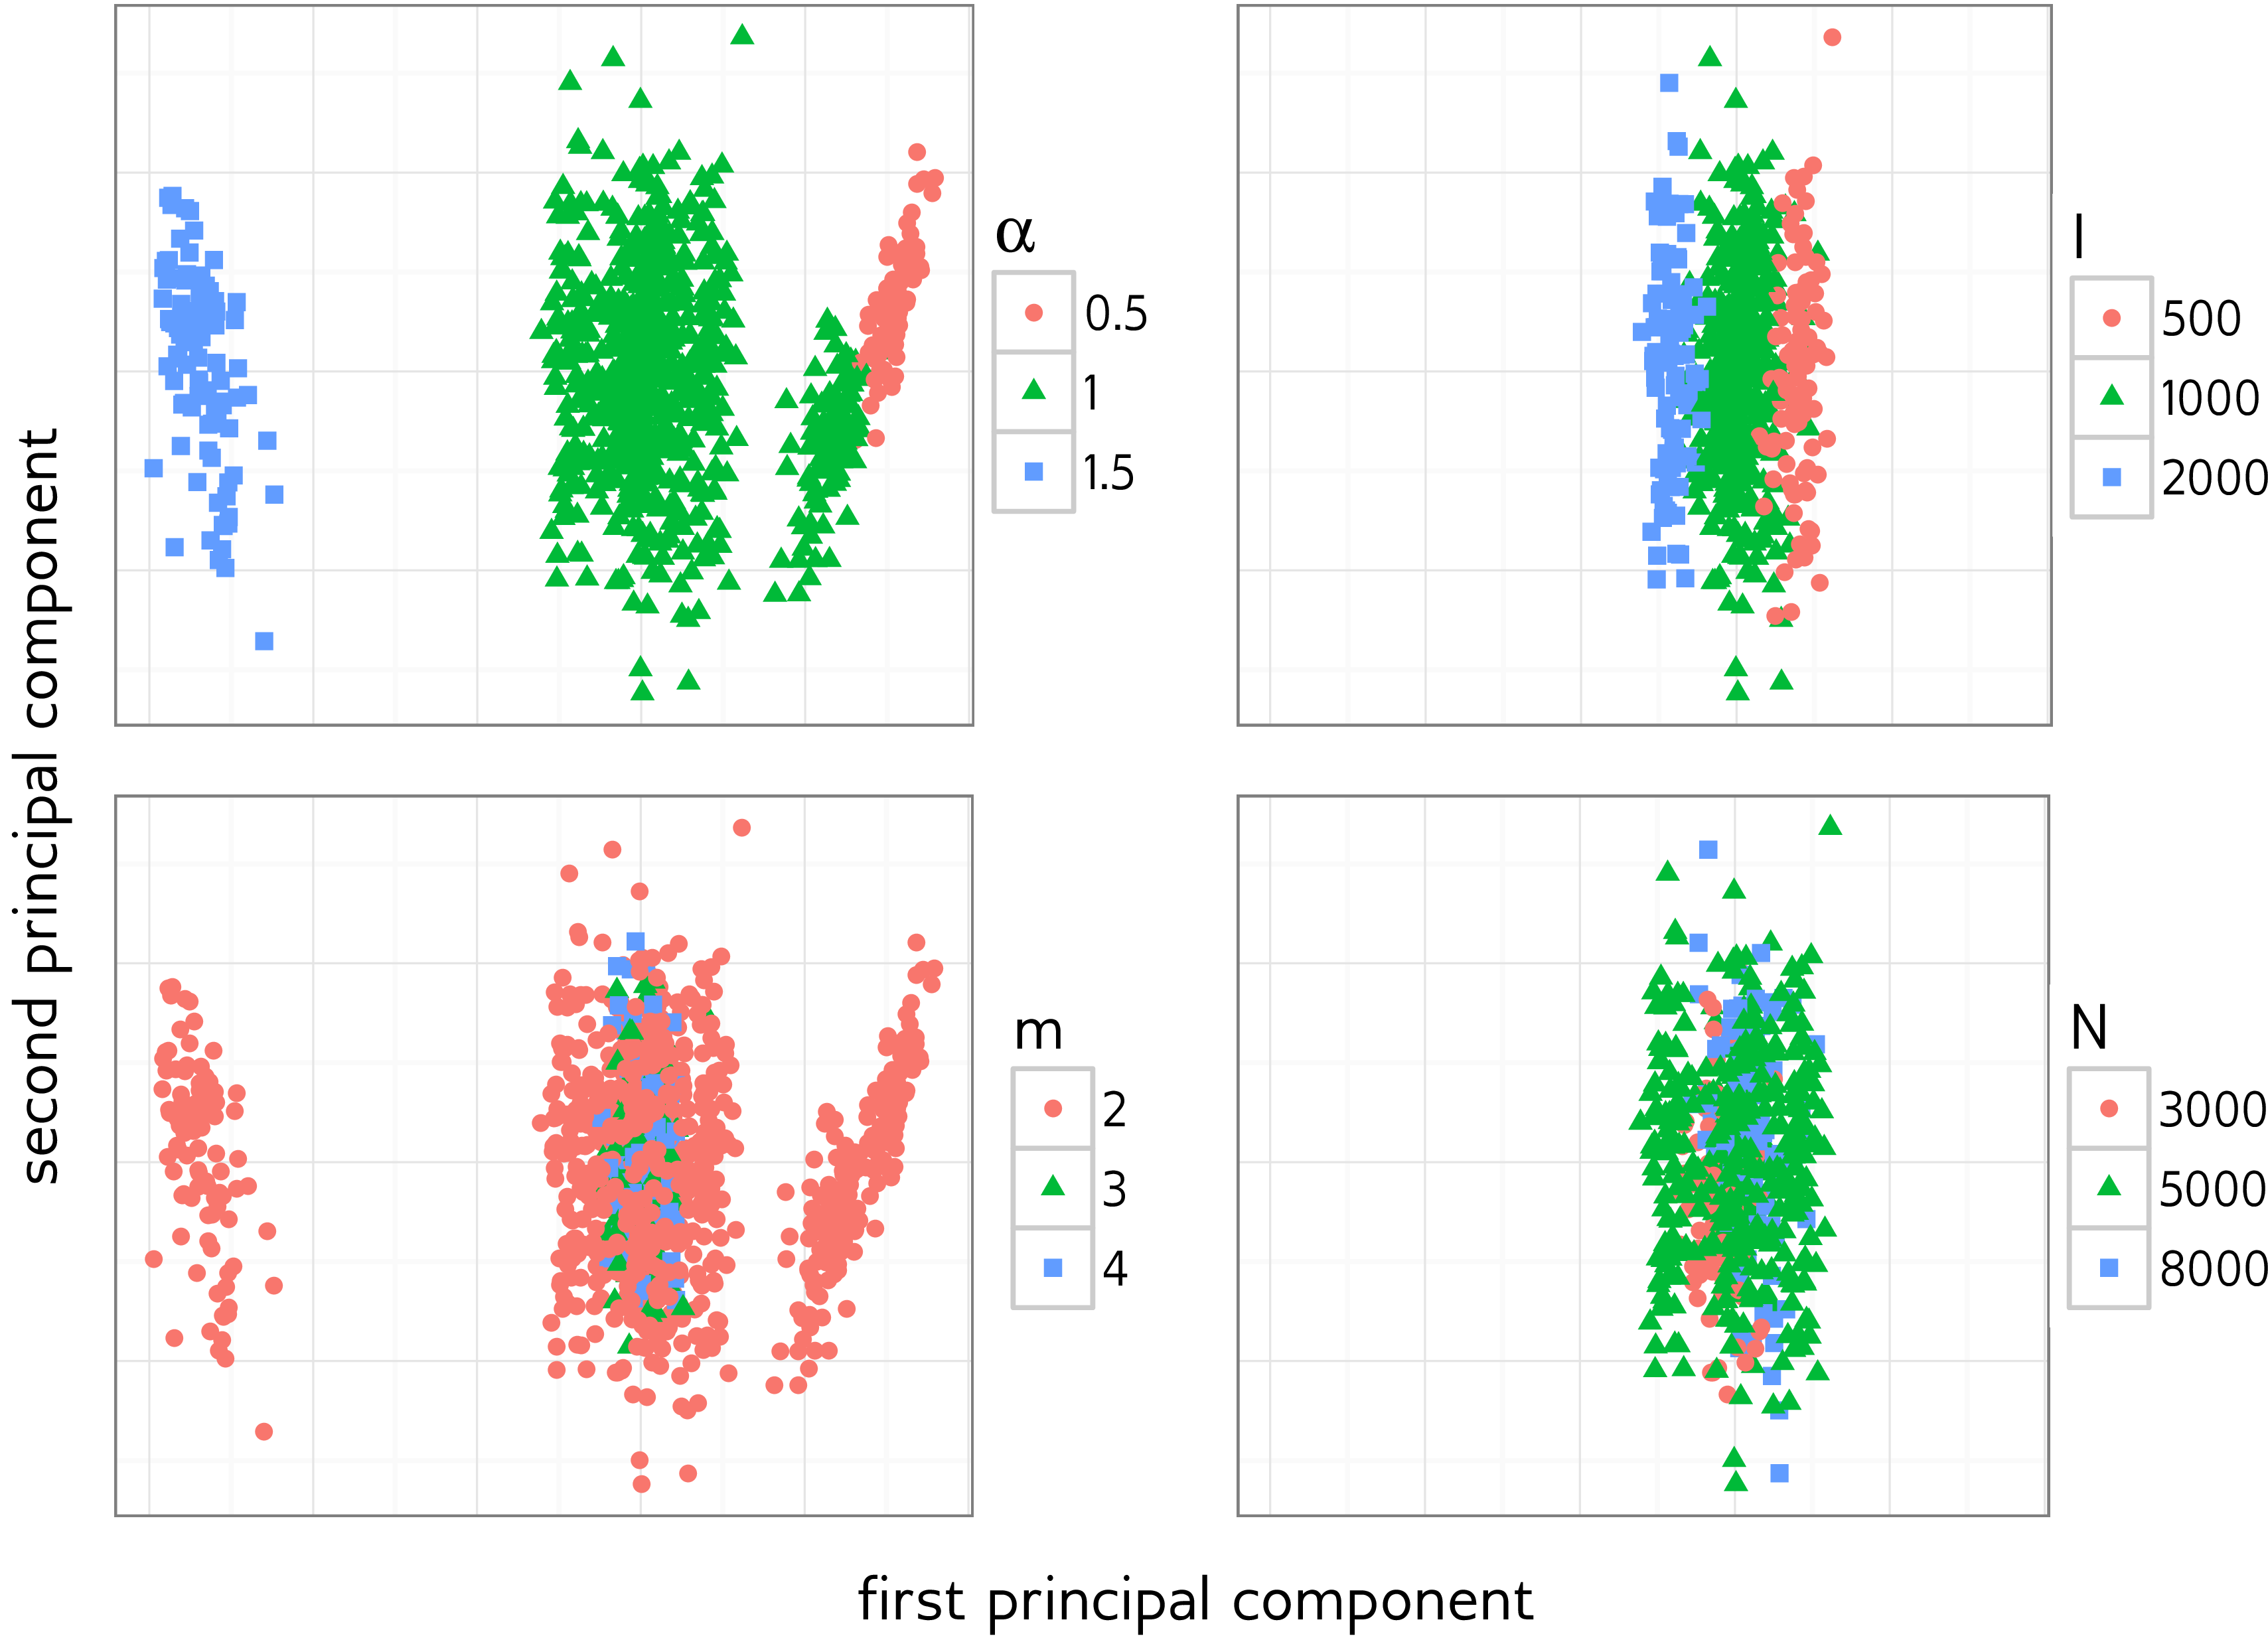
\includegraphics[width=0.6\textwidth, trim=3.5in 0.3in 0 2.2in, clip]{kernel-kpca.pdf}};
    \node (t) at (current page.north east) [anchor=north east, inner ysep=1.5cm, inner xsep=0.5cm] {\includegraphics[width=0.7\textwidth]{kernel-N-tree.pdf}};
  \end{tikzpicture}
\end{frame}

\begin{frame}{Simulated trees can be used to fit a network model}
  \begin{minipage}[p][\textheight][t]{\textwidth}
    \only<1>{\includegraphics[width=0.9\textwidth, trim=0 3in 0 0, clip]{abc-idea.pdf}}
    \only<2>{\includegraphics[width=0.9\textwidth, trim=0 1.8in 0 0, clip]{abc-idea.pdf}}
    \only<3>{\includegraphics[width=0.9\textwidth, trim=0 1in 0 0, clip]{abc-idea.pdf}}
    \uncover<4->{\includegraphics[width=0.9\textwidth, trim=0 0in 0 0, clip]{abc-idea.pdf}}
    \uncover<5->{\vspace{0.5cm}\centerline{\textbf{kernel approximate Bayesian computation (kernel-ABC)}}}
  \end{minipage}
\end{frame}

\begin{frame}{Example simulation shows $\alpha$ and $I$ can be reconstructed}
  \begin{minipage}[p][\textheight][t]{\textwidth}
    \begin{center}
    preferential attachment power \hfill prevalence
    \only<1>{
      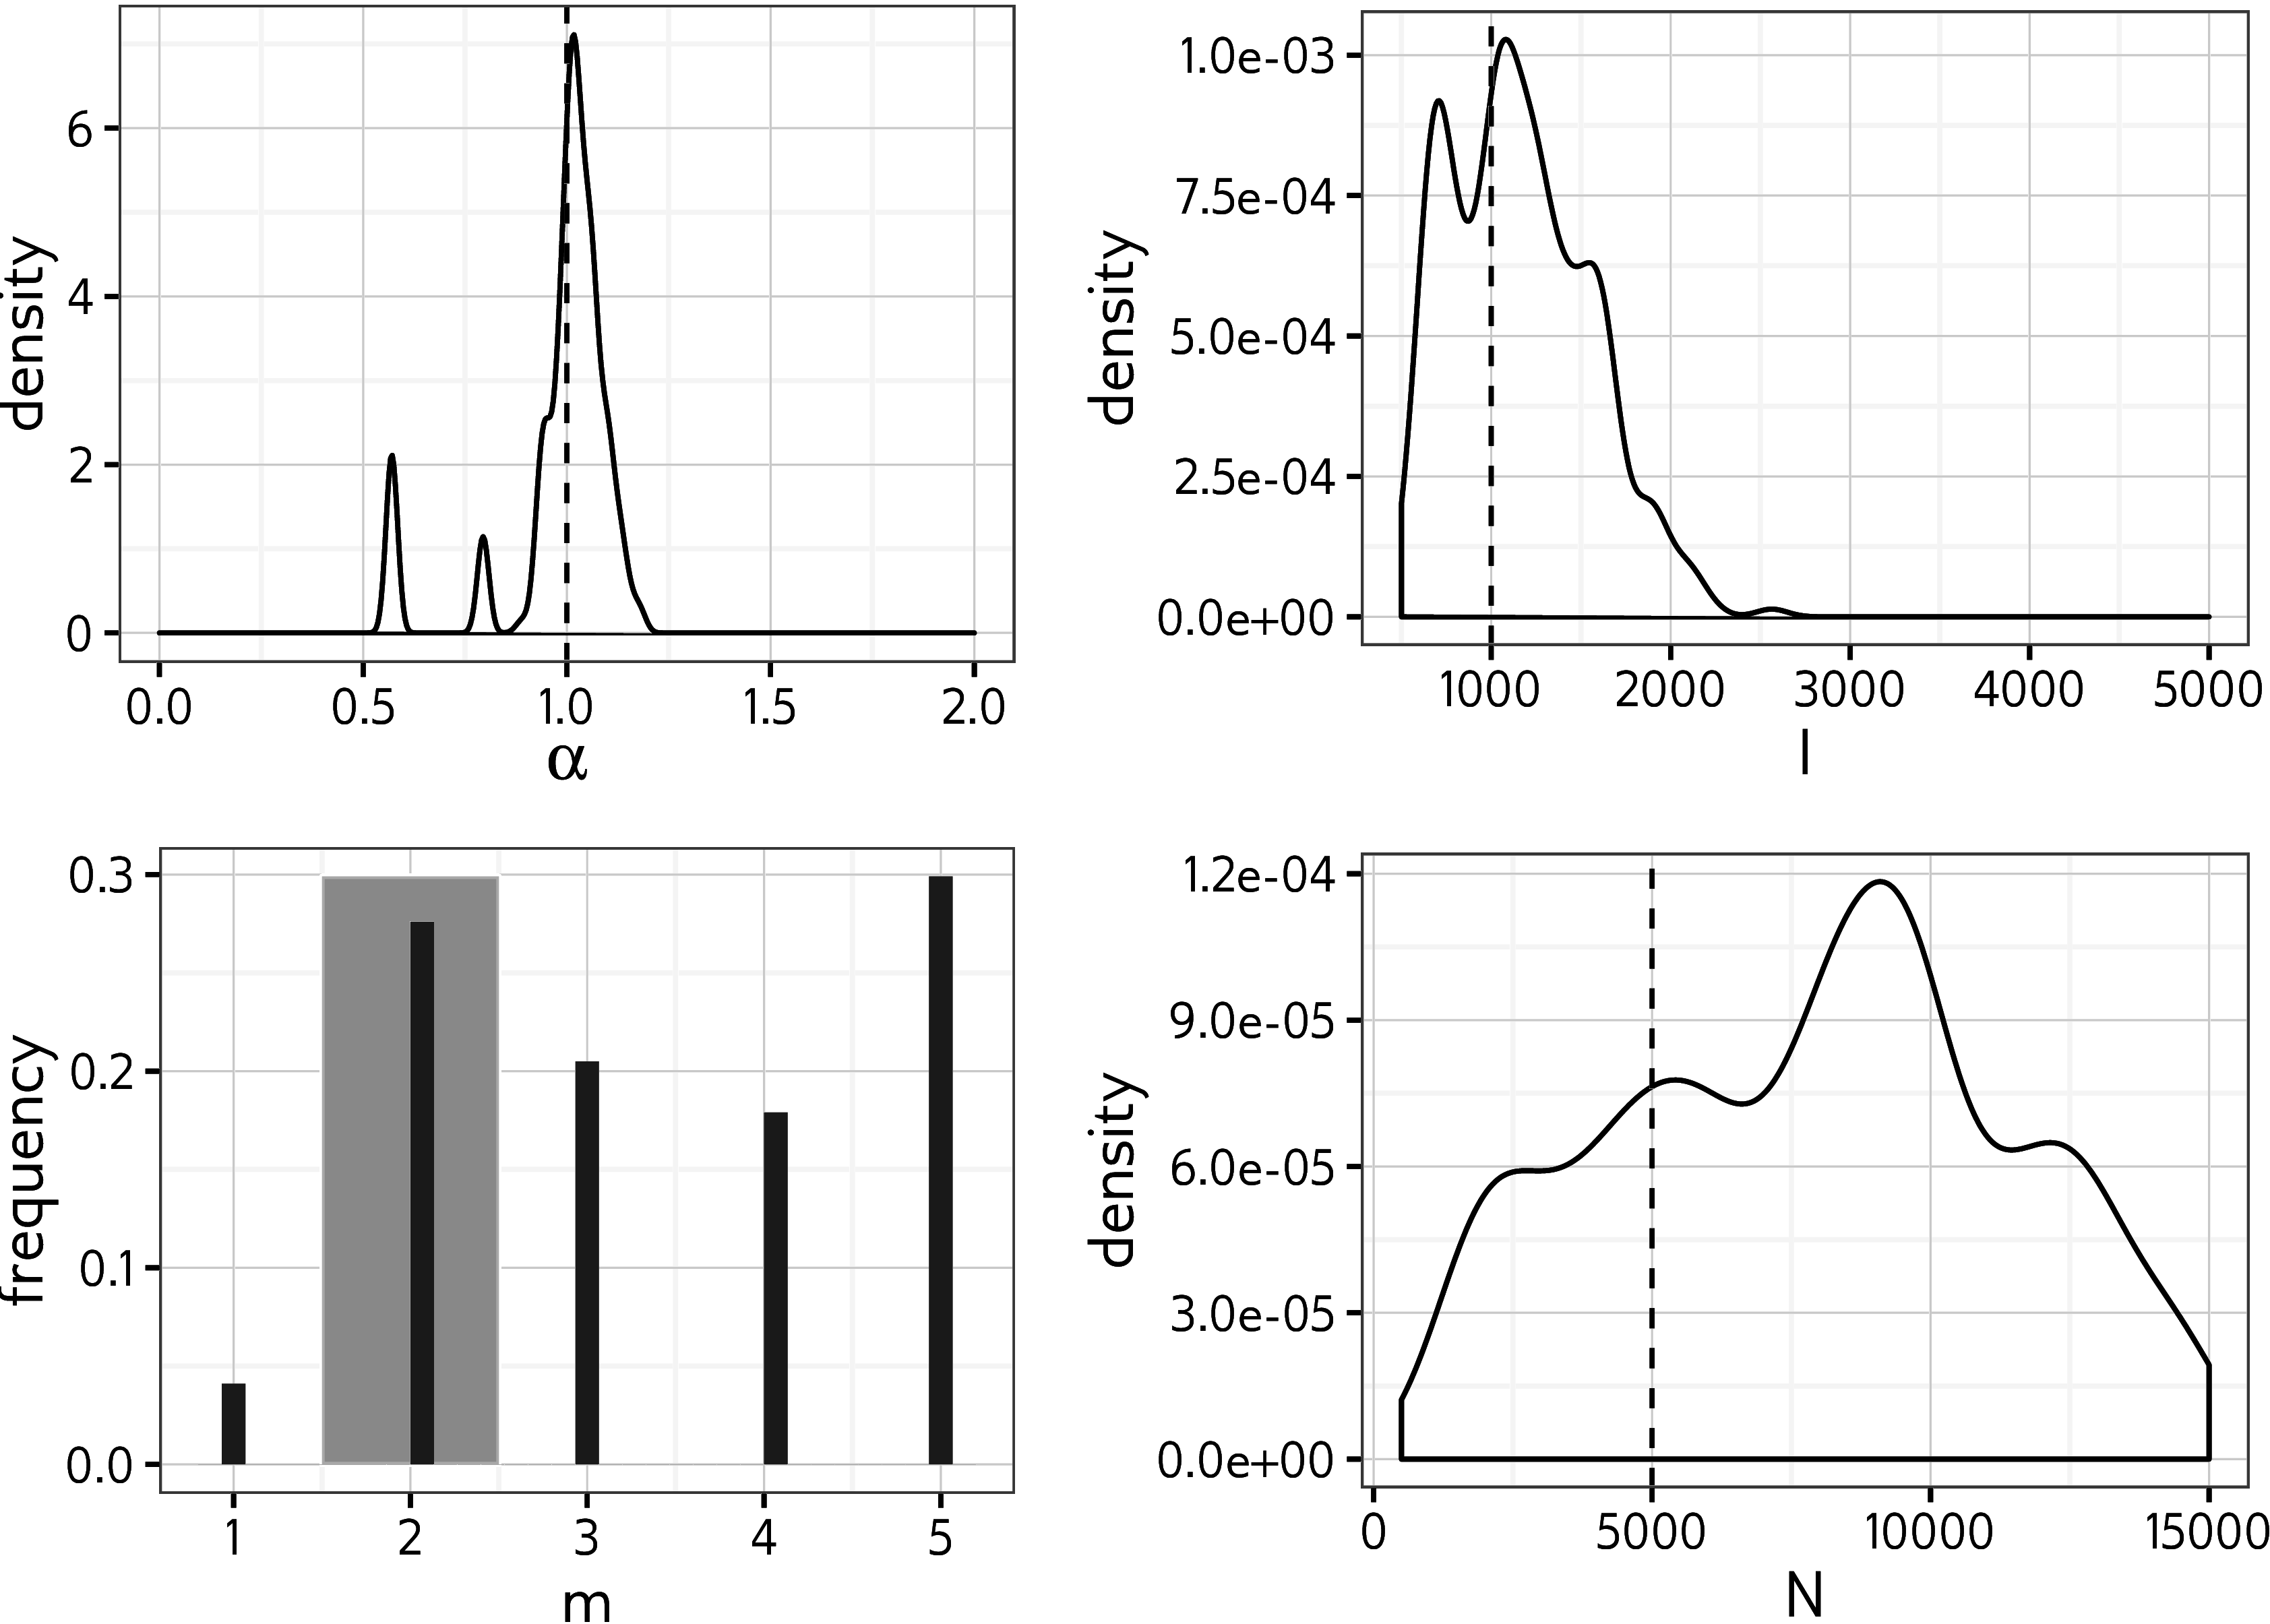
\includegraphics[width=0.8\textwidth, trim=0 2.5in 0 0, clip]{abc-posterior-example.pdf}
    }
    \only<2>{
      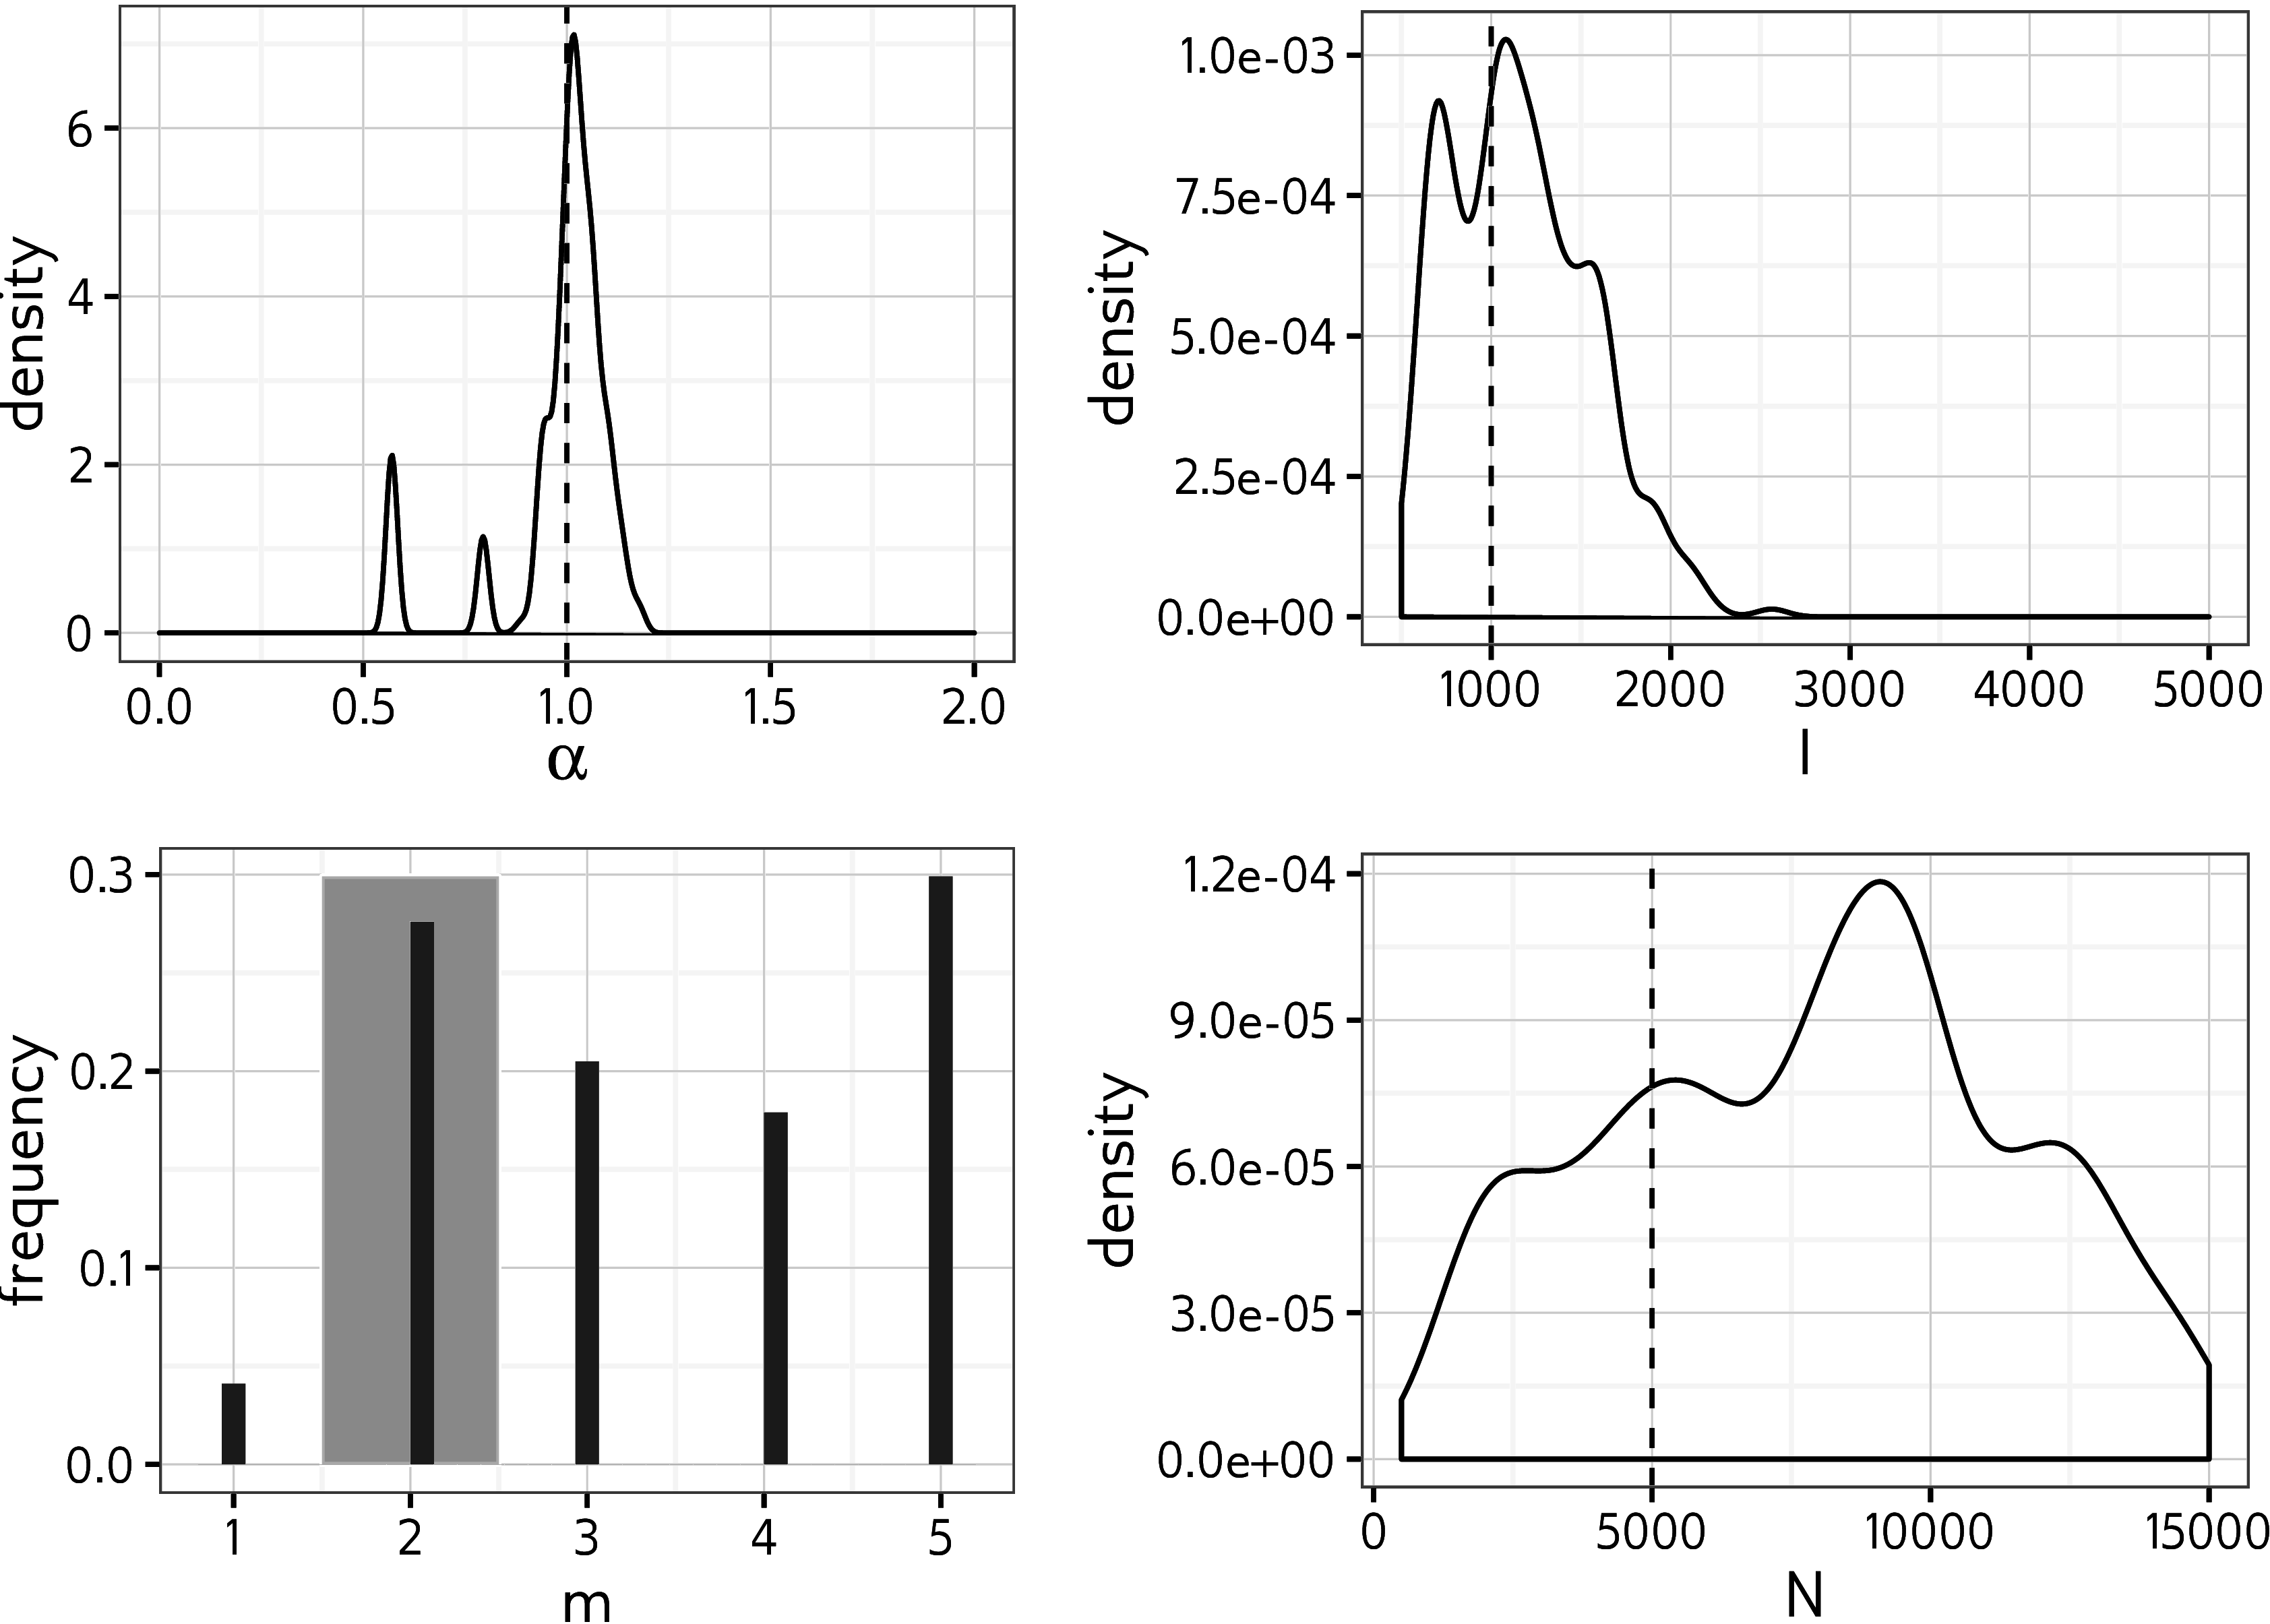
\includegraphics[width=0.8\textwidth]{abc-posterior-example.pdf}

      \vspace{-0.25cm}
      edges per vertex \hfill total nodes
    }
    \end{center}
  \end{minipage}
\end{frame}

\begin{frame}{Maximum \textit{a posteriori} estimates are accurate for $\alpha$ and $I$}
  \begin{minipage}[p][\textheight][t]{\textwidth}
    \vspace{-0.5cm}
    preferential attachment power \hfill \uncover<2>{edges per vertex}

    \hspace{0.75cm}\only<1>{\includegraphics[height=0.8\textheight, trim=0 0 3.4in 0, clip]{abc-point-estimate-m2.pdf}}
    \only<2>{\includegraphics[height=0.8\textheight]{abc-point-estimate-m2.pdf}}

    prevalence \hfill \uncover<2>{total nodes}
  \end{minipage}
\end{frame}

\begin{frame}{Real world HIV datasets exhibit network heterogeneity}
  \uncover<2->{
    \centerline{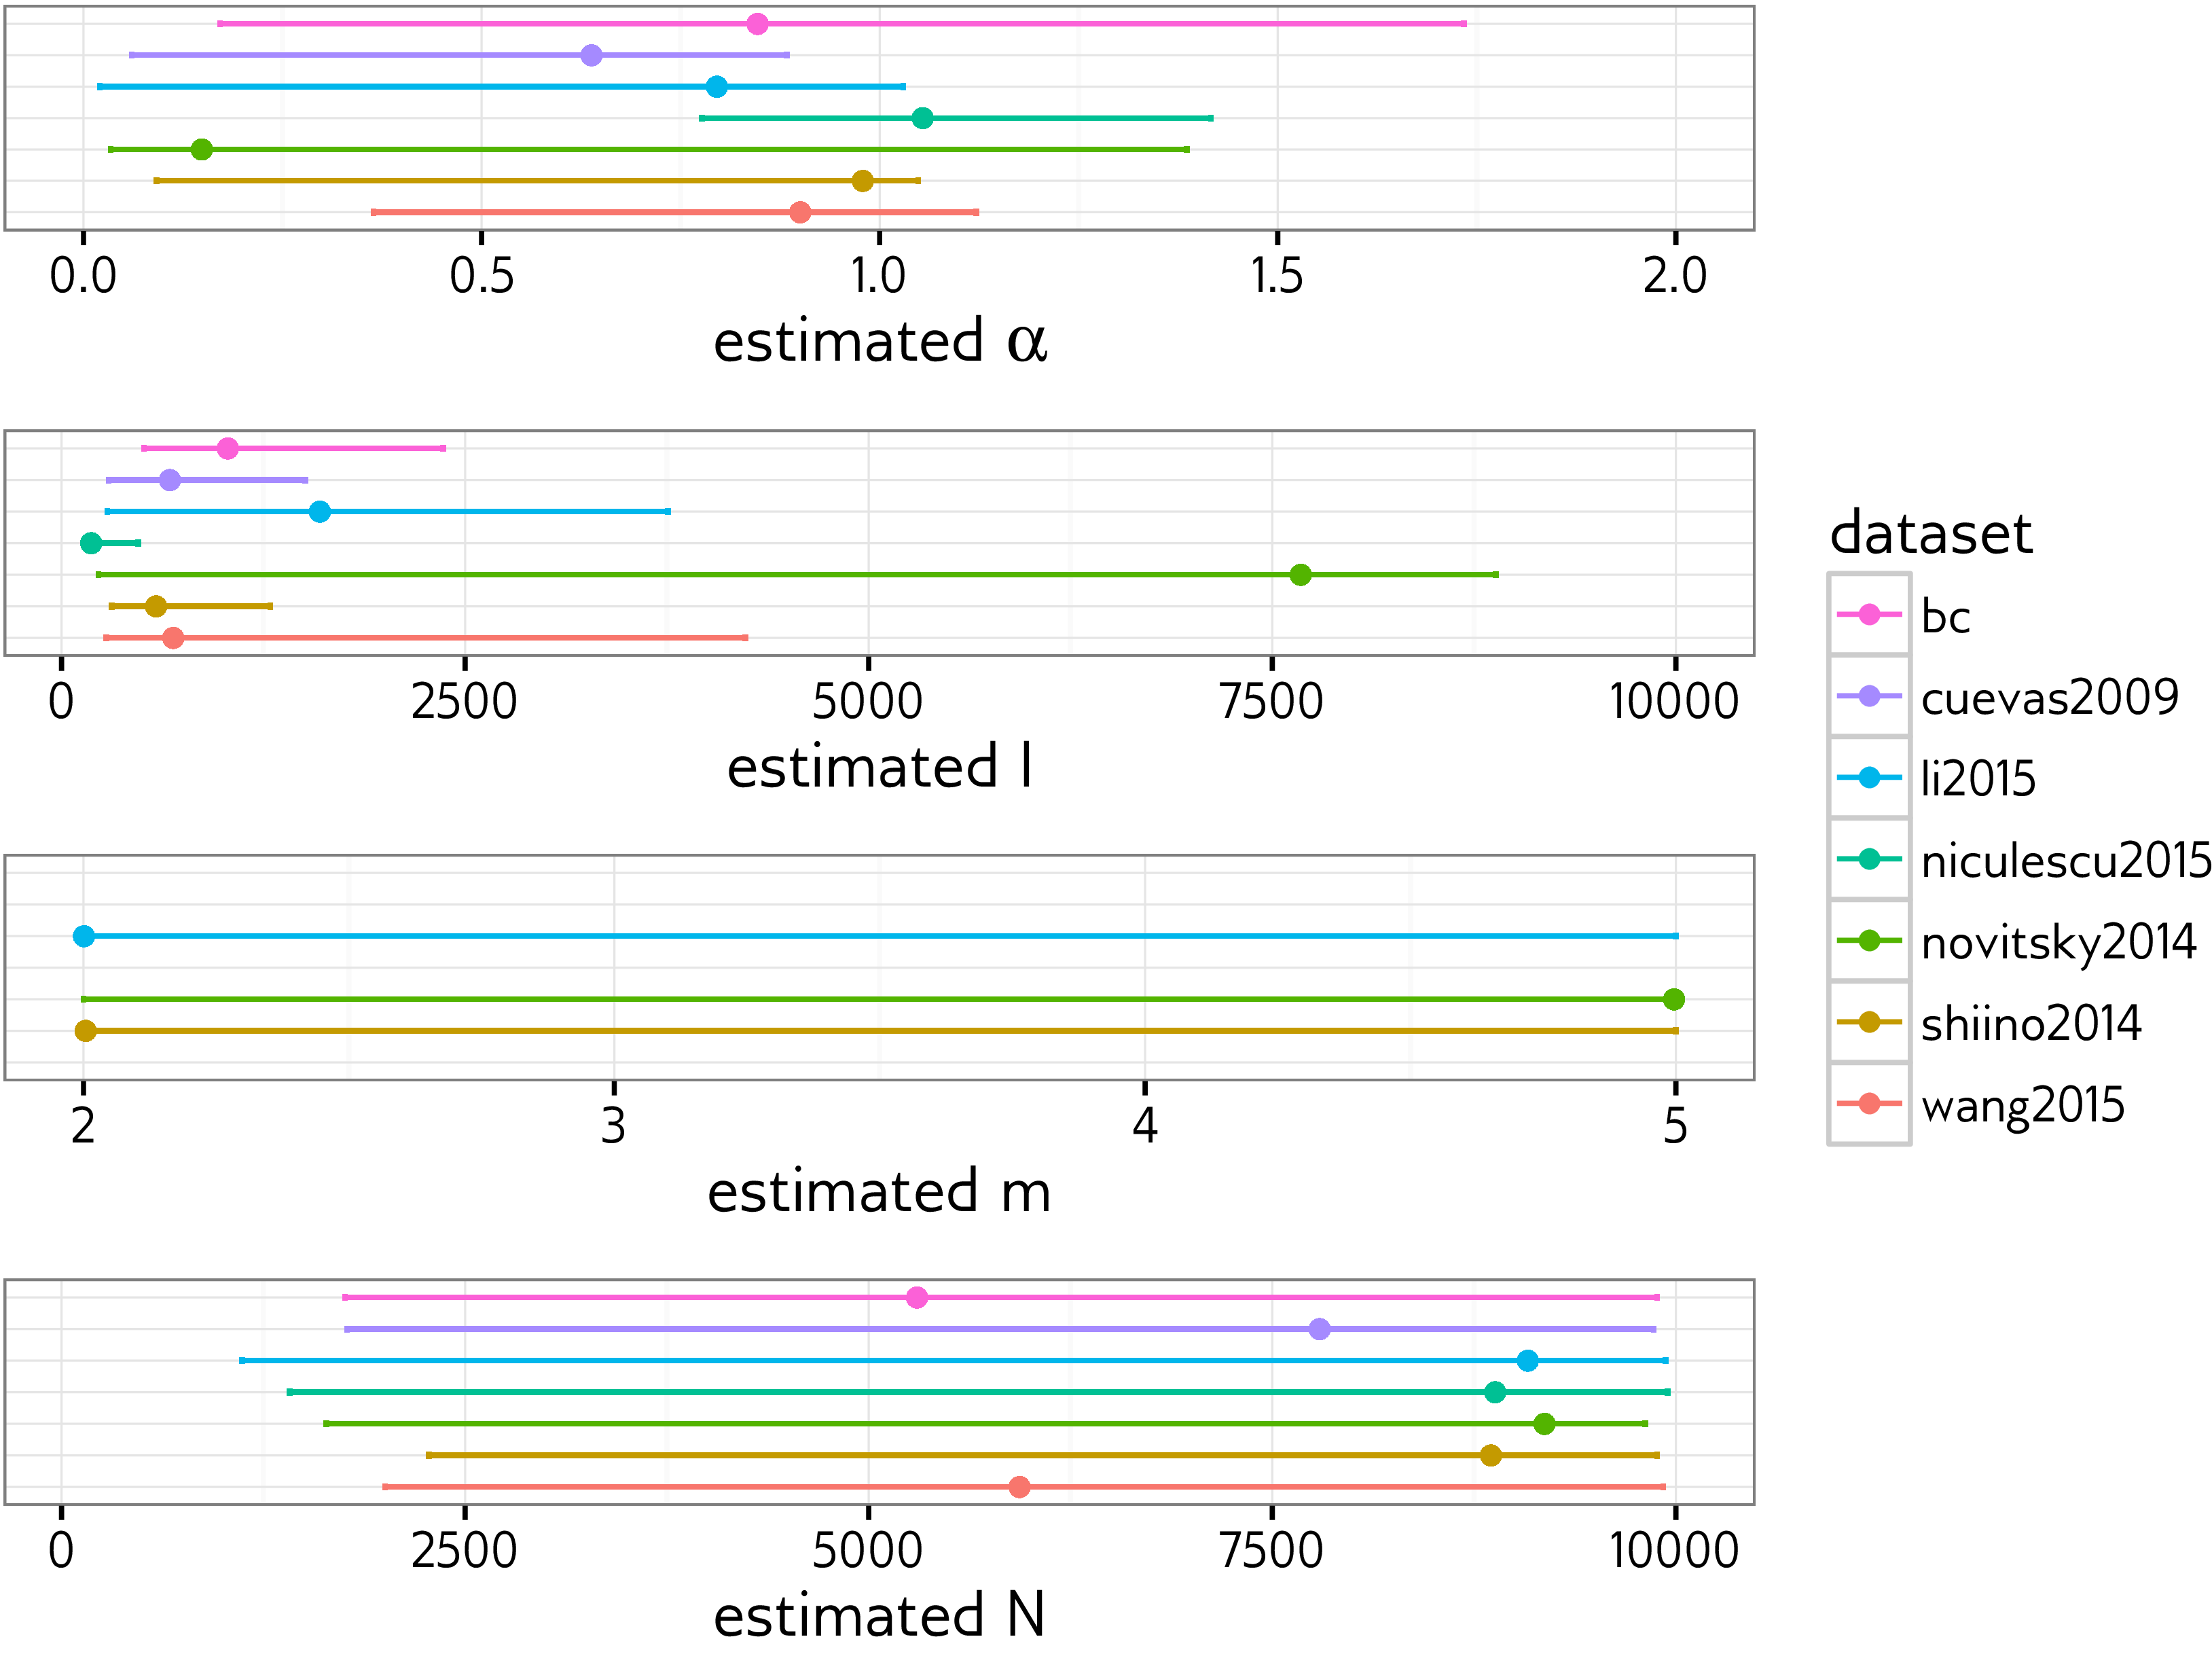
\includegraphics[height=0.8\textheight]{realdata-hpd-bc}}
  }

%  \scriptsize
%    \begin{tabular}{ccccc}
%      Reference & Sequences ($n$) & Location & Risk group & Gene \\
%      \hline
%      \color{magenta} \textcite{novitsky2013phylogenetic} &
%        \color{magenta} \multirow{2}{*}{180} &
%        \color{magenta} \multirow{2}{*}{Mochudi, Botswana} & 
%        \color{magenta} \multirow{2}{*}{HET} &
%        \color{magenta} \multirow{2}{*}{\textit{env}} \\ 
%      \color{magenta} \textcite{novitsky2014impact} \\
%      \color{blue} \textcite{cuevas2009hiv} & 
%        \color{blue} 287 & 
%        \color{blue} Basque Country, Spain & 
%        \color{blue} mixed & 
%        \color{blue} \textit{pol} \\
%      \color{cyan} \textcite{li2015hiv} & 
%        \color{cyan} 280 & 
%        \color{cyan} Shanghai, China & 
%        \color{cyan} MSM & 
%        \color{cyan} \textit{pol} \\
%      \color{green} unpublished & 
%        \color{green} 399 & 
%        \color{green} British Columbia, Canada & 
%        \color{green} IDU & 
%        \color{green} \textit{pol} \\
%      \color{orange} \textcite{wang2015targeting} & 
%        \color{orange} 173 & 
%        \color{orange} Beijing, China & 
%        \color{orange} MSM & 
%        \color{orange} \textit{pol} \\
%      \color{red} \textcite{niculescu2015recent} & 
%        \color{red} 136 & 
%        \color{red} Romaina & 
%        \color{red} IDU & 
%        \color{red} \textit{pol} \\
%      \hline
%    \end{tabular}
%  \normalsize
\end{frame}

\begin{frame}{Conclusions}
  \begin{itemize}
    \item Kernel-ABC is the first phylodynamic method to fit contact network
      models to phylogenetic data.
      \pause
    \item The preferential attachment power of the Barab\'asi-Albert network
      model, which is challenging to estimate by traditional epidemiological
      methods, can be estimated with kernel-ABC.
      \pause
    \item The networks underlying real epidemics are heterogeneous,
      underscoring the importance of considering network structure in
      phylodynamic analyses.
      \pause
  \end{itemize}
  \centerline{\qrcode{github.com/rmcclosk/netabc} github.com/rmcclosk/netabc}
\end{frame}

\begin{frame}{Acknowledgements}
  \begin{columns}
    \begin{column}{0.6\textwidth}

      \textbf{BC Centre for Excellence in HIV/AIDS}

      Art Poon

      Jeff Joy

      Richard Liang

      Thuy Nguyen

      P. Richard Harrigan

      \hfill\\
      \textbf{University of British Columbia}

      Sarah Otto

      Alexandre Bouchard-C\^ot\'e

      \vfill
      \vspace{0.5cm}
      $\qquad\qquad$
\includegraphics[width=2cm]{logos/genomecanada}
      $\qquad$
      
\includegraphics[width=2cm]{logos/genomequebec}
    \end{column}
    \begin{column}{0.4\textwidth}
      \centering 

      
\includegraphics[width=3cm]{logos/cfe}
      \vspace{0.5cm}

      
\includegraphics[width=3cm]{logos/cihr}

      
\includegraphics[width=3cm]{logos/genomebc}

      
\includegraphics[width=3cm]{logos/bmgf}
      \vspace{0.5cm}

      
\includegraphics[width=3cm]{logos/btp}
    \end{column}
  \end{columns}
\end{frame}

\begin{frame}{Classifiers for network parameters}
  \vspace{-1cm}
  \begin{itemize}
    \item kSVR using tree kernel
    \item SVR using normalized
      lineages-through-time\footfullcite{janzen2015approximate}
    \item linear regression using Sackin's index~\footfullcite{shao1990tree}
  \end{itemize}

  \includegraphics[width=\textwidth]{kernel-rsquared.pdf}
\end{frame}

\begin{frame}{Sequential Monte Carlo for ABC}
  \begin{tikzpicture}
    \only<1-2>{\node at (0, 0) [anchor=north west] {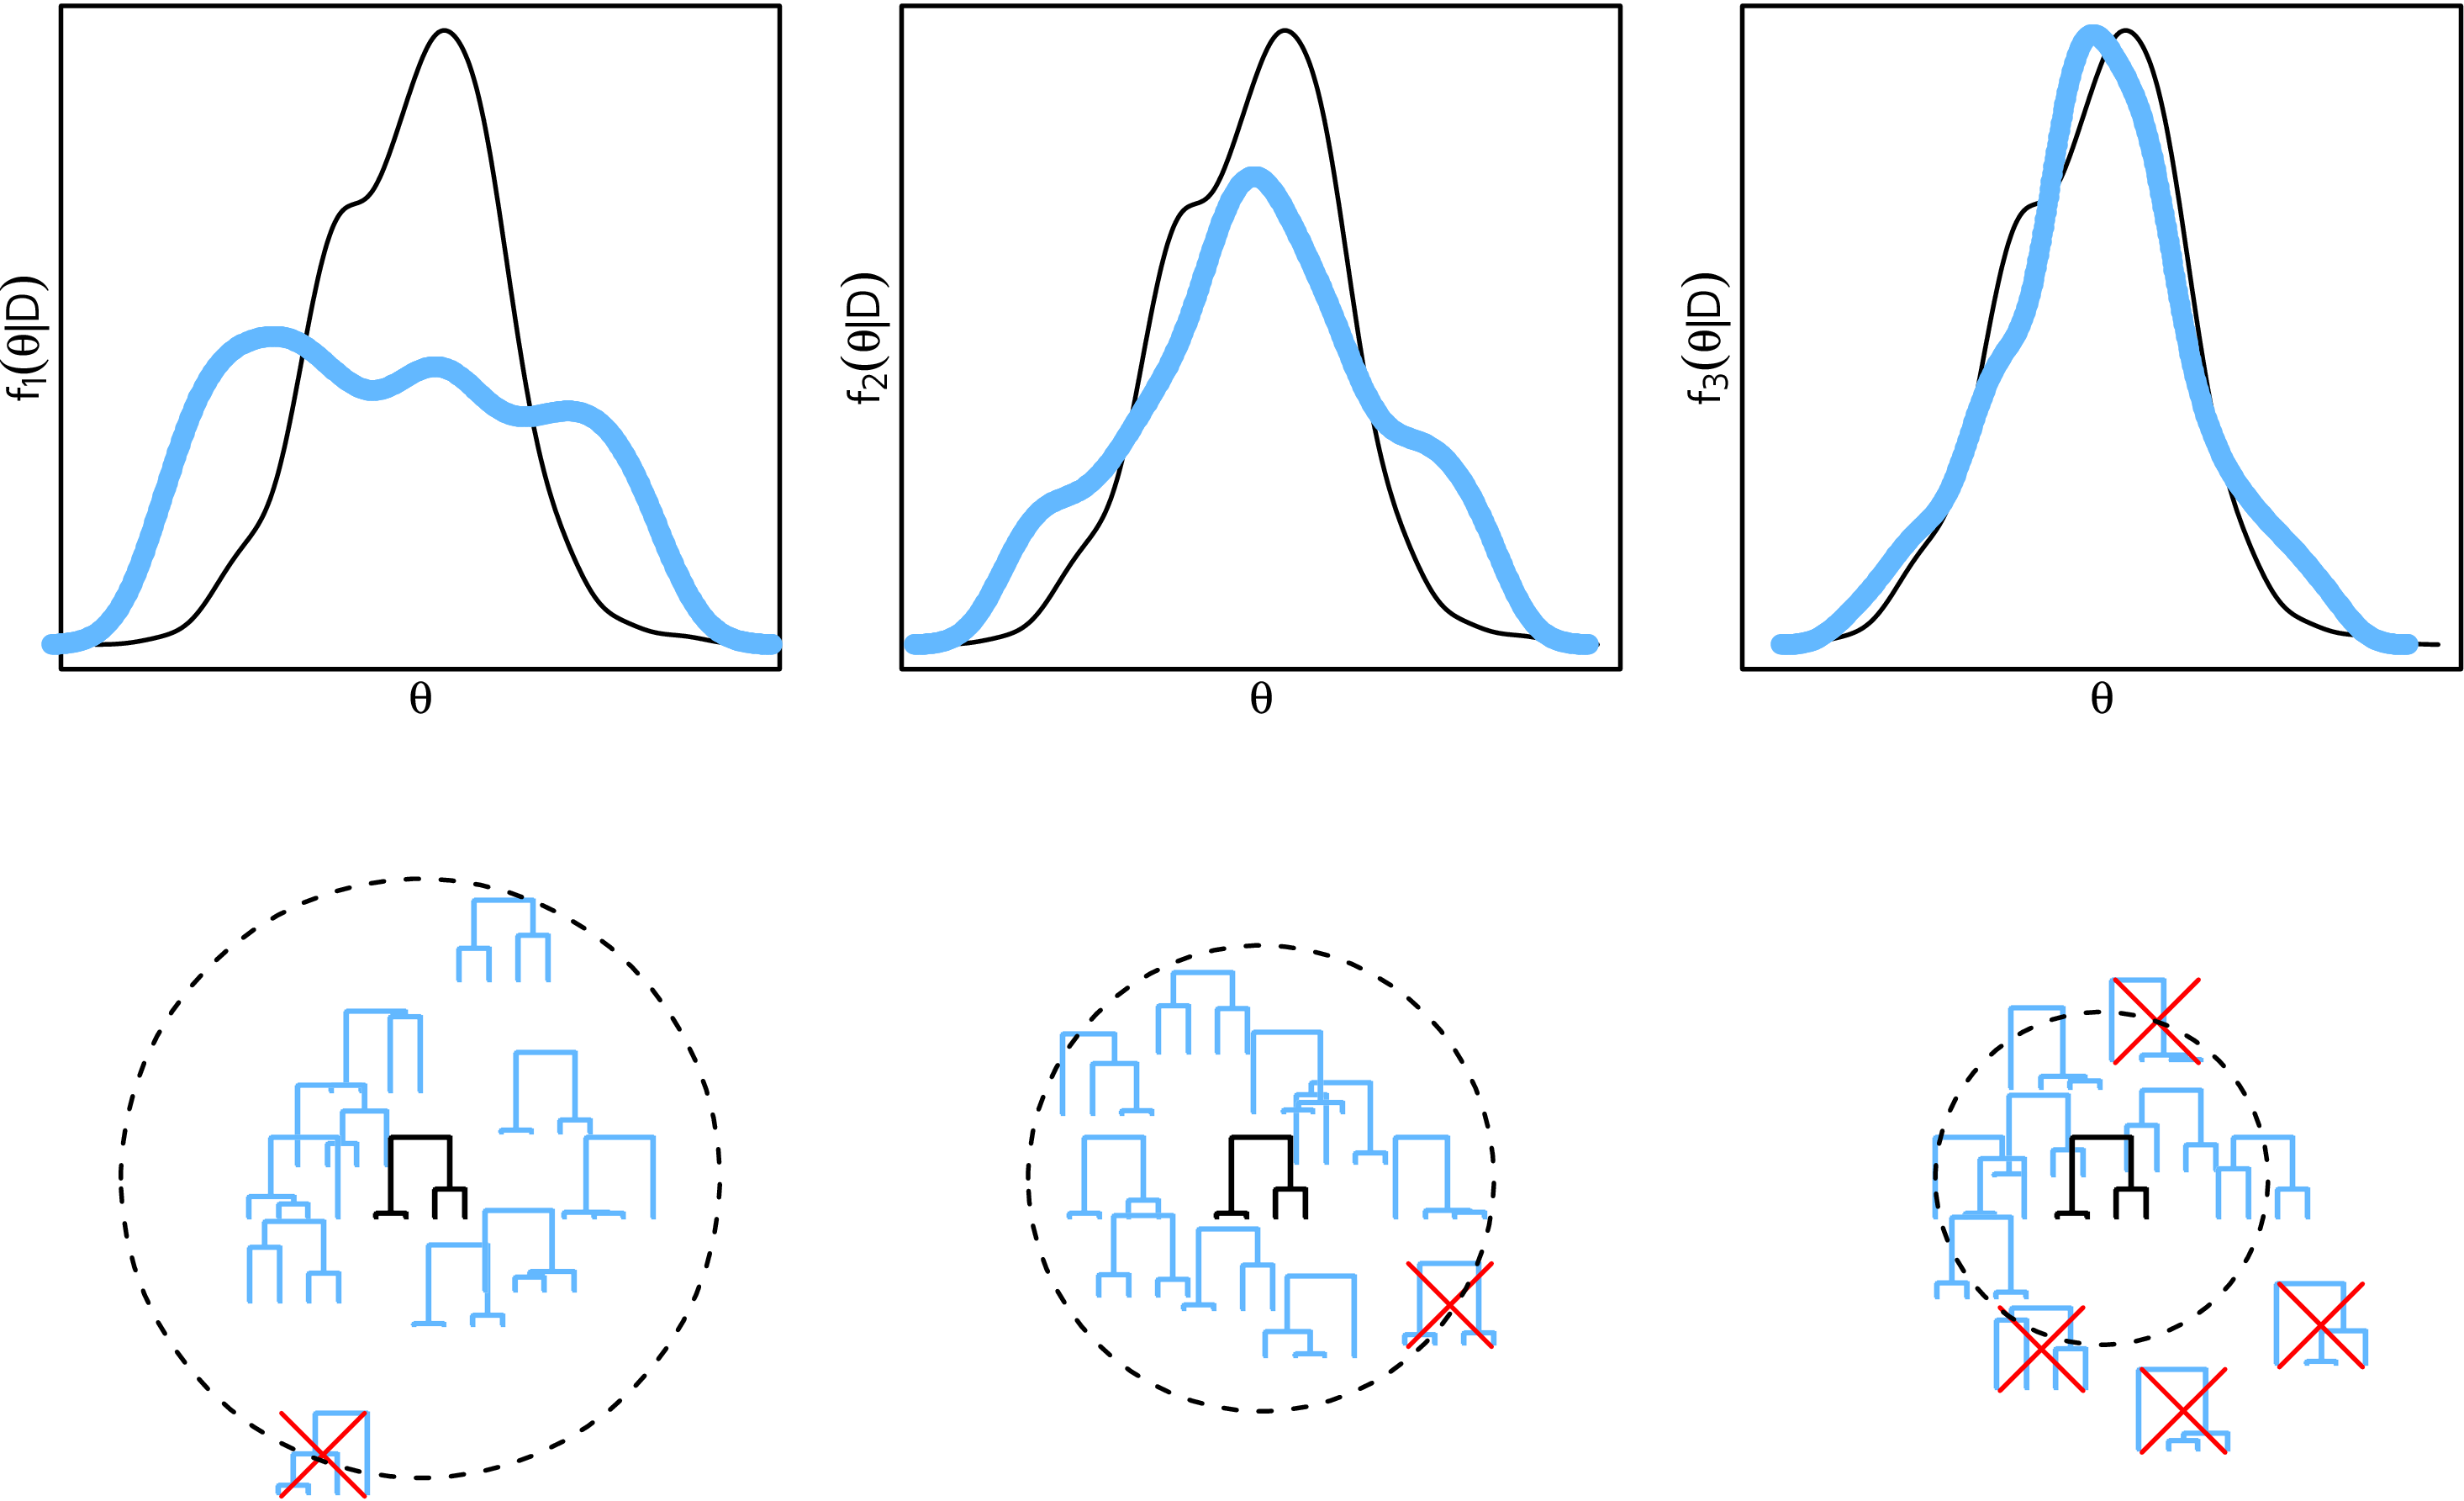
\includegraphics[height=0.7\textheight, trim=0 0in 4in 0, clip]{abc-smc.pdf}}};
    \only<1>{\fill[white] (0.2,-6.5) rectangle (4,-3.5)};
    \only<3>{\node at (0, 0) [anchor=north west] {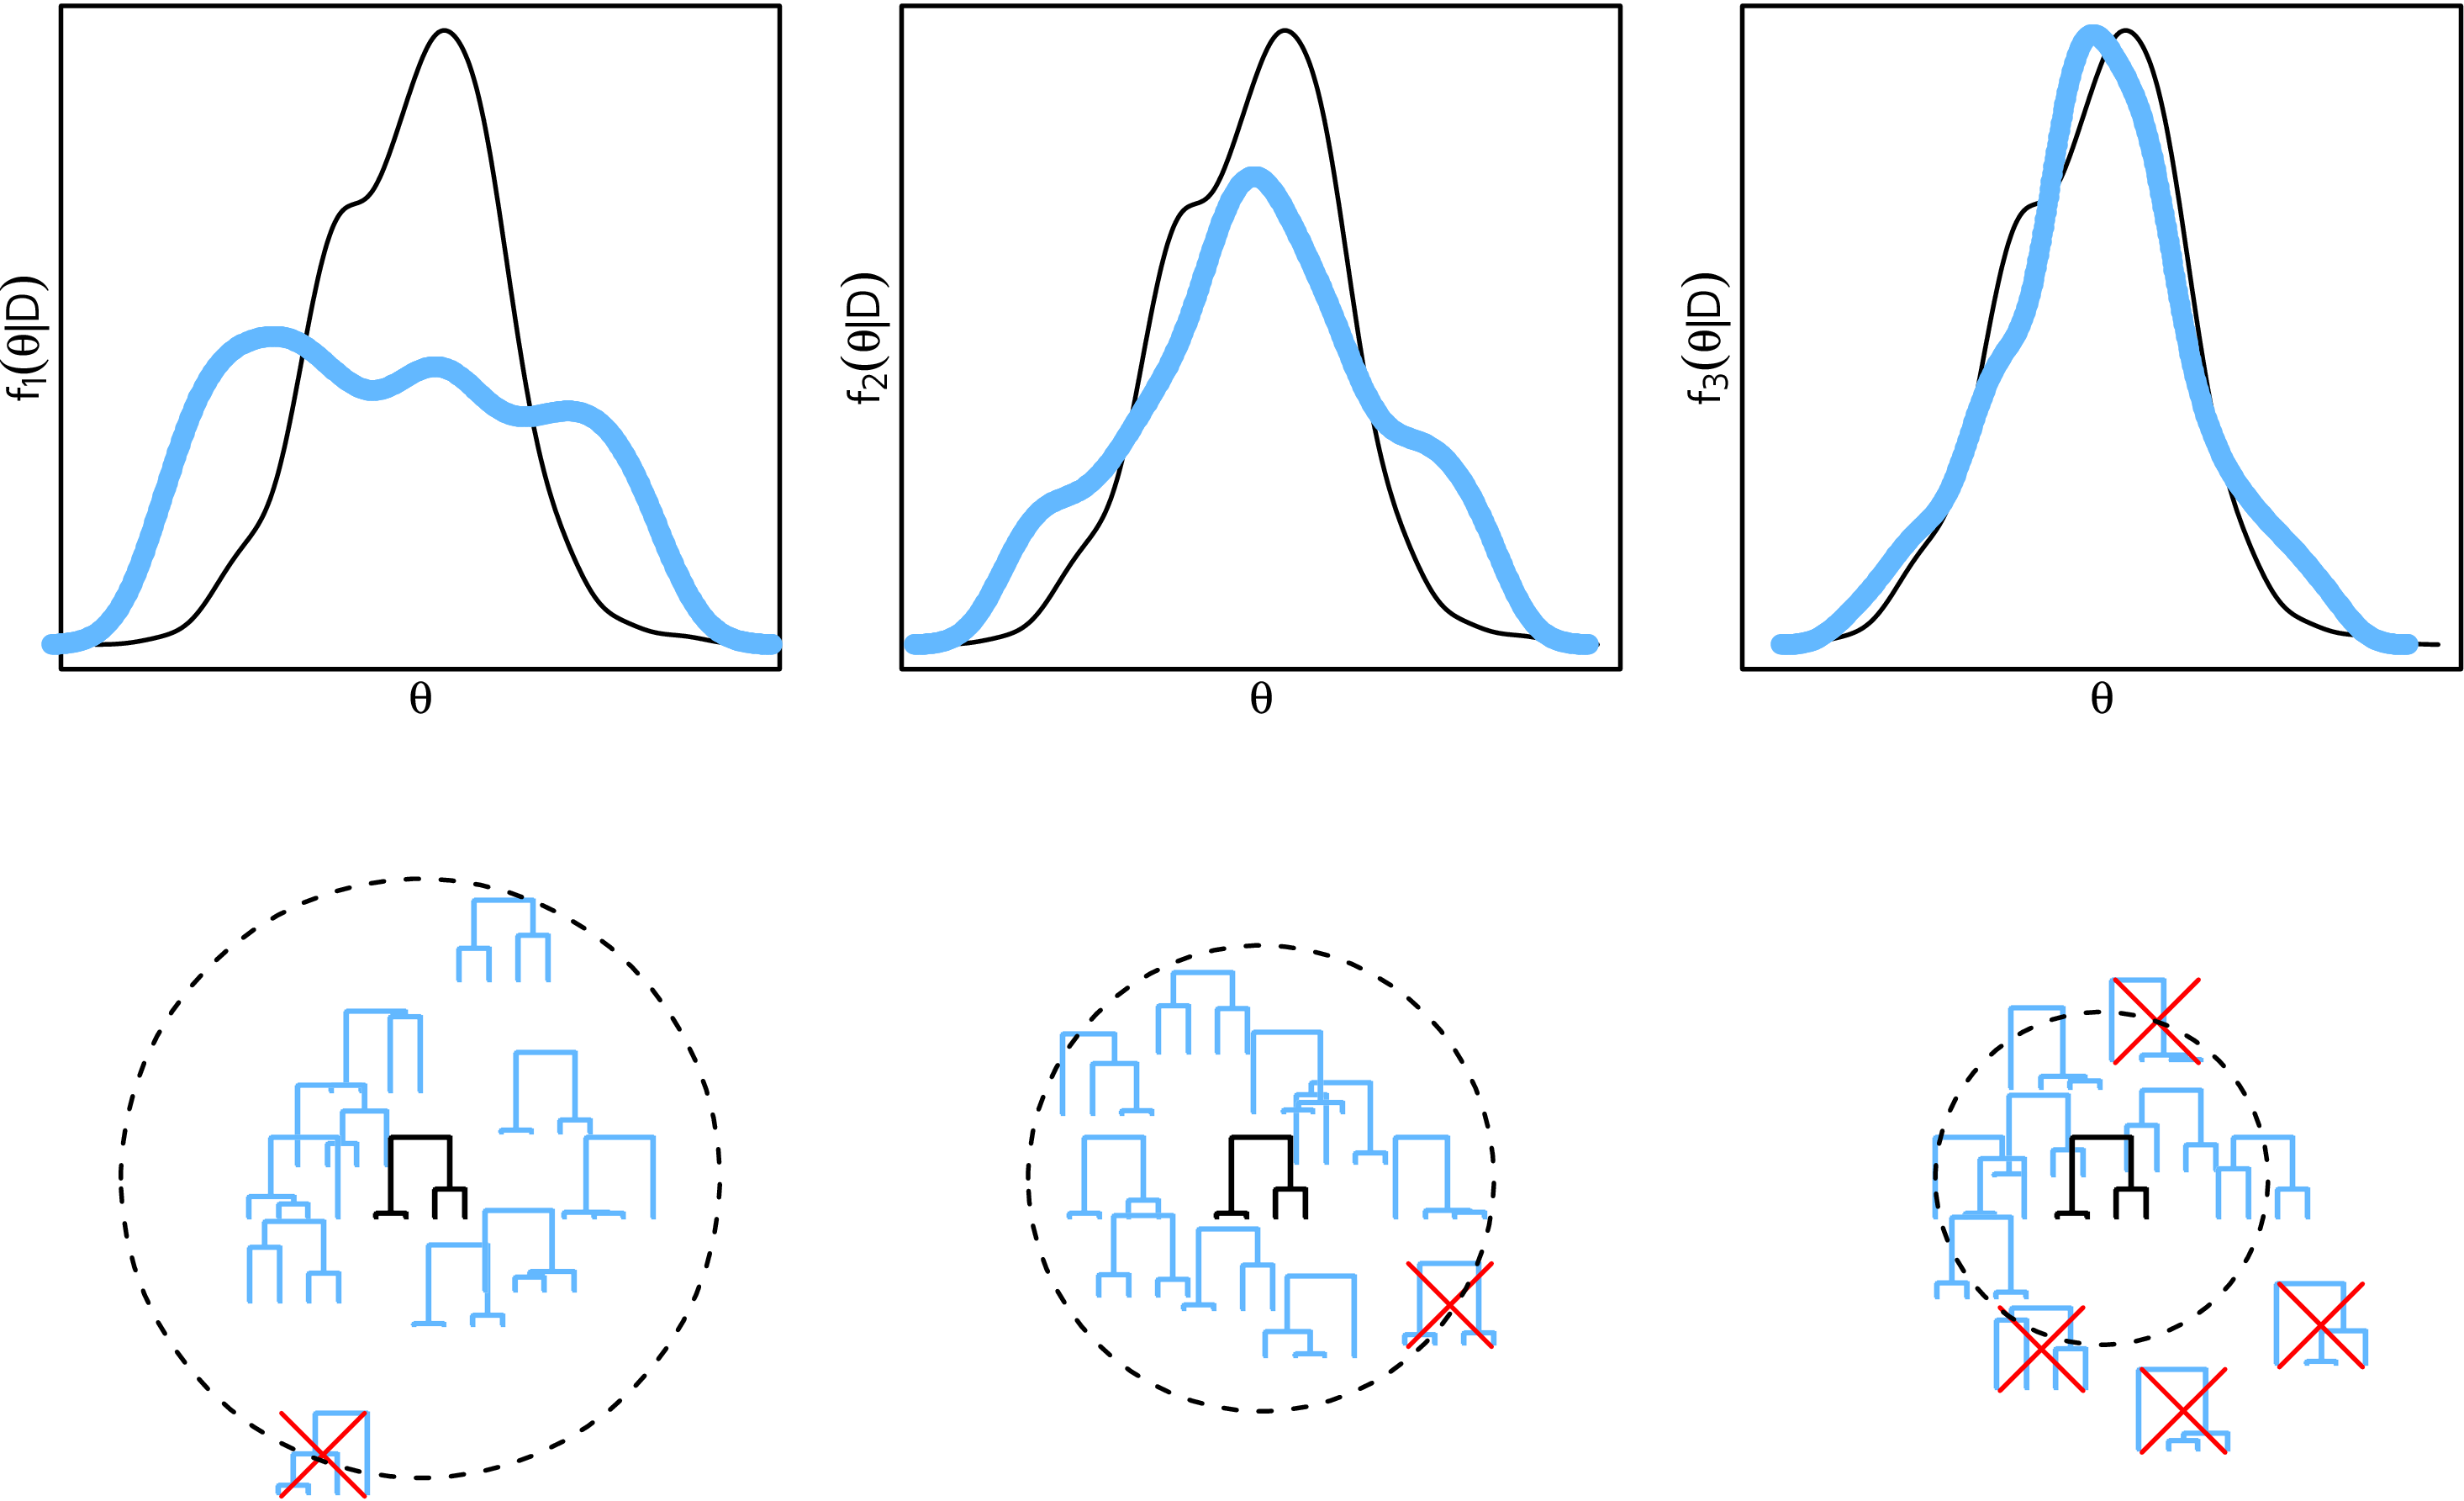
\includegraphics[height=0.7\textheight, trim=0 0in 2in 0, clip]{abc-smc.pdf}}};
    \only<4>{\node at (0, 0) [anchor=north west] {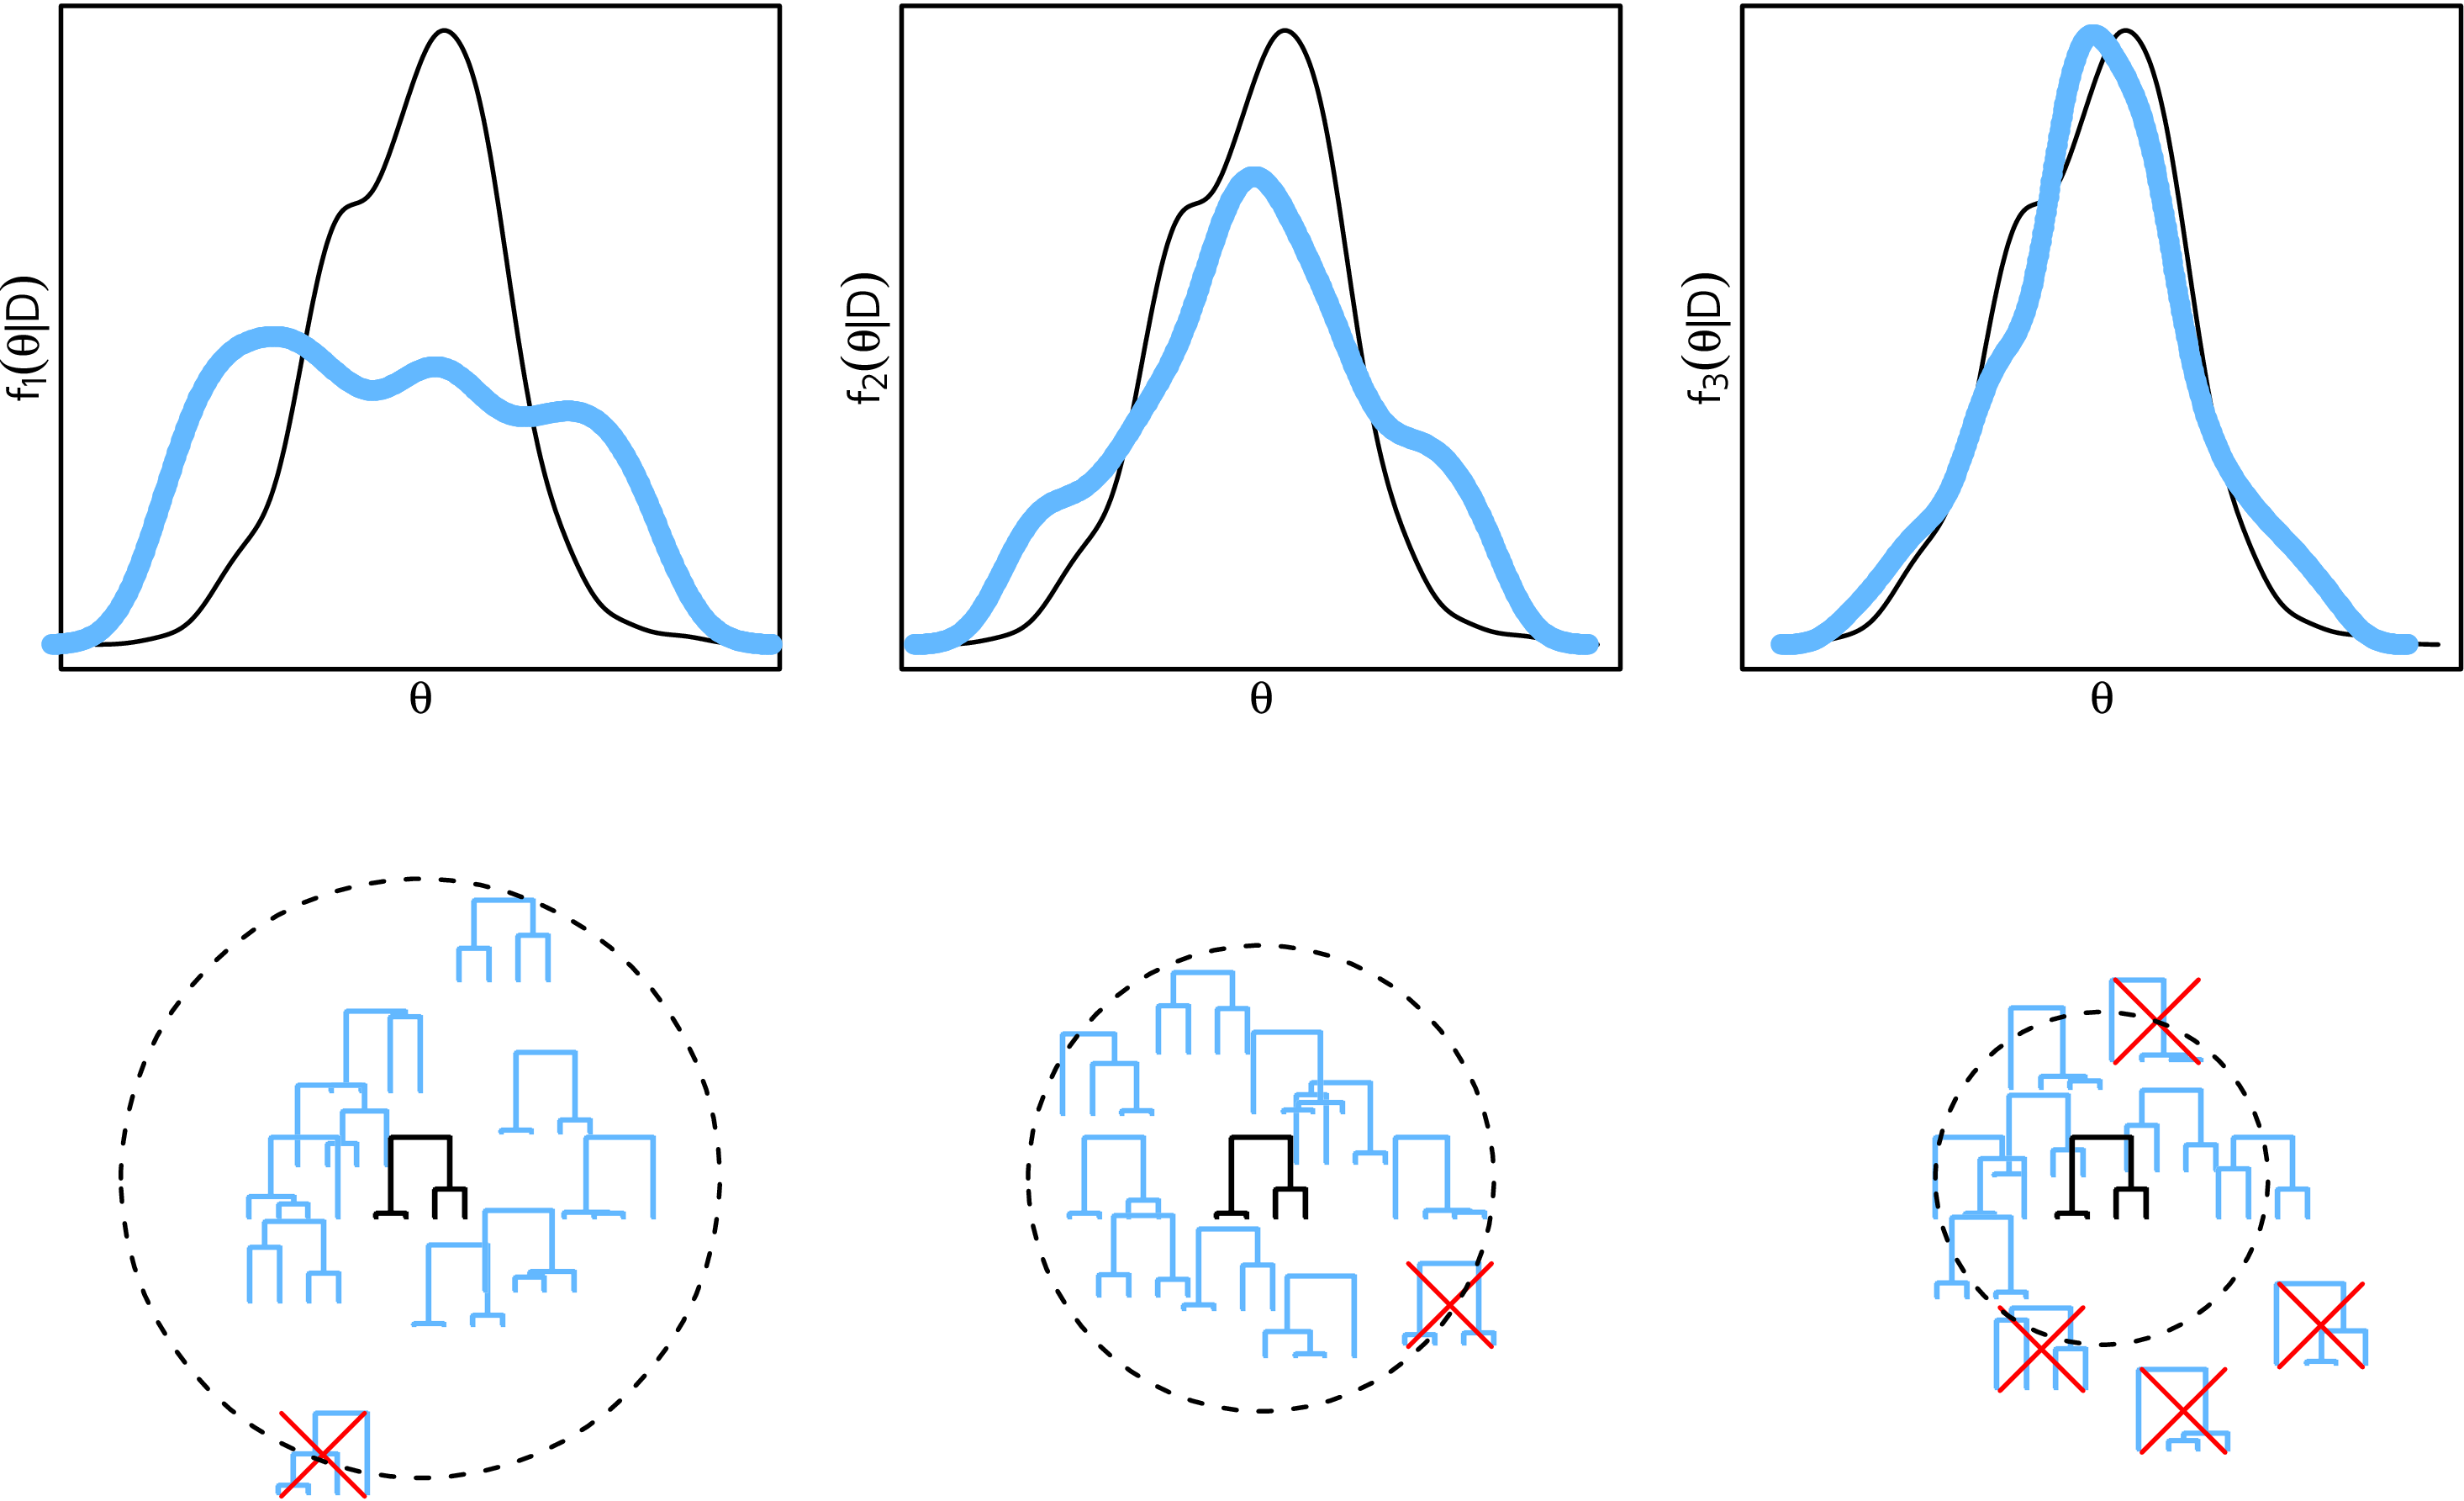
\includegraphics[height=0.7\textheight, trim=0 0in 0 0, clip]{abc-smc.pdf}}};
  \end{tikzpicture}
\end{frame}


\end{document}
